% Options for packages loaded elsewhere
\PassOptionsToPackage{unicode}{hyperref}
\PassOptionsToPackage{hyphens}{url}
\PassOptionsToPackage{dvipsnames,svgnames,x11names}{xcolor}
%
\documentclass[
  12pt,
]{article}

\usepackage{amsmath,amssymb}
\usepackage{lmodern}
\usepackage{setspace}
\usepackage{iftex}
\ifPDFTeX
  \usepackage[T1]{fontenc}
  \usepackage[utf8]{inputenc}
  \usepackage{textcomp} % provide euro and other symbols
\else % if luatex or xetex
  \usepackage{unicode-math}
  \defaultfontfeatures{Scale=MatchLowercase}
  \defaultfontfeatures[\rmfamily]{Ligatures=TeX,Scale=1}
\fi
% Use upquote if available, for straight quotes in verbatim environments
\IfFileExists{upquote.sty}{\usepackage{upquote}}{}
\IfFileExists{microtype.sty}{% use microtype if available
  \usepackage[]{microtype}
  \UseMicrotypeSet[protrusion]{basicmath} % disable protrusion for tt fonts
}{}
\makeatletter
\@ifundefined{KOMAClassName}{% if non-KOMA class
  \IfFileExists{parskip.sty}{%
    \usepackage{parskip}
  }{% else
    \setlength{\parindent}{0pt}
    \setlength{\parskip}{6pt plus 2pt minus 1pt}}
}{% if KOMA class
  \KOMAoptions{parskip=half}}
\makeatother
\usepackage{xcolor}
\usepackage[top=30mm,left=25mm,right=25mm,heightrounded]{geometry}
\setlength{\emergencystretch}{3em} % prevent overfull lines
\setcounter{secnumdepth}{5}
% Make \paragraph and \subparagraph free-standing
\ifx\paragraph\undefined\else
  \let\oldparagraph\paragraph
  \renewcommand{\paragraph}[1]{\oldparagraph{#1}\mbox{}}
\fi
\ifx\subparagraph\undefined\else
  \let\oldsubparagraph\subparagraph
  \renewcommand{\subparagraph}[1]{\oldsubparagraph{#1}\mbox{}}
\fi


\providecommand{\tightlist}{%
  \setlength{\itemsep}{0pt}\setlength{\parskip}{0pt}}\usepackage{longtable,booktabs,array}
\usepackage{calc} % for calculating minipage widths
% Correct order of tables after \paragraph or \subparagraph
\usepackage{etoolbox}
\makeatletter
\patchcmd\longtable{\par}{\if@noskipsec\mbox{}\fi\par}{}{}
\makeatother
% Allow footnotes in longtable head/foot
\IfFileExists{footnotehyper.sty}{\usepackage{footnotehyper}}{\usepackage{footnote}}
\makesavenoteenv{longtable}
\usepackage{graphicx}
\makeatletter
\def\maxwidth{\ifdim\Gin@nat@width>\linewidth\linewidth\else\Gin@nat@width\fi}
\def\maxheight{\ifdim\Gin@nat@height>\textheight\textheight\else\Gin@nat@height\fi}
\makeatother
% Scale images if necessary, so that they will not overflow the page
% margins by default, and it is still possible to overwrite the defaults
% using explicit options in \includegraphics[width, height, ...]{}
\setkeys{Gin}{width=\maxwidth,height=\maxheight,keepaspectratio}
% Set default figure placement to htbp
\makeatletter
\def\fps@figure{htbp}
\makeatother
\newlength{\cslhangindent}
\setlength{\cslhangindent}{1.5em}
\newlength{\csllabelwidth}
\setlength{\csllabelwidth}{3em}
\newlength{\cslentryspacingunit} % times entry-spacing
\setlength{\cslentryspacingunit}{\parskip}
\newenvironment{CSLReferences}[2] % #1 hanging-ident, #2 entry spacing
 {% don't indent paragraphs
  \setlength{\parindent}{0pt}
  % turn on hanging indent if param 1 is 1
  \ifodd #1
  \let\oldpar\par
  \def\par{\hangindent=\cslhangindent\oldpar}
  \fi
  % set entry spacing
  \setlength{\parskip}{#2\cslentryspacingunit}
 }%
 {}
\usepackage{calc}
\newcommand{\CSLBlock}[1]{#1\hfill\break}
\newcommand{\CSLLeftMargin}[1]{\parbox[t]{\csllabelwidth}{#1}}
\newcommand{\CSLRightInline}[1]{\parbox[t]{\linewidth - \csllabelwidth}{#1}\break}
\newcommand{\CSLIndent}[1]{\hspace{\cslhangindent}#1}

\usepackage{booktabs}
\usepackage{longtable}
\usepackage{array}
\usepackage{multirow}
\usepackage{wrapfig}
\usepackage{float}
\usepackage{colortbl}
\usepackage{pdflscape}
\usepackage{tabu}
\usepackage{threeparttable}
\usepackage{threeparttablex}
\usepackage[normalem]{ulem}
\usepackage{makecell}
\usepackage{xcolor}
\usepackage{lineno}
\usepackage[noblocks]{authblk}
\renewcommand*{\Authsep}{, }
\renewcommand*{\Authand}{, }
\renewcommand*{\Authands}{, }
\renewcommand\Affilfont{\small}
\usepackage{setspace}
\makeatletter
\makeatother
\makeatletter
\makeatother
\makeatletter
\@ifpackageloaded{caption}{}{\usepackage{caption}}
\AtBeginDocument{%
\ifdefined\contentsname
  \renewcommand*\contentsname{Table of contents}
\else
  \newcommand\contentsname{Table of contents}
\fi
\ifdefined\listfigurename
  \renewcommand*\listfigurename{List of Figures}
\else
  \newcommand\listfigurename{List of Figures}
\fi
\ifdefined\listtablename
  \renewcommand*\listtablename{List of Tables}
\else
  \newcommand\listtablename{List of Tables}
\fi
\ifdefined\figurename
  \renewcommand*\figurename{Figure}
\else
  \newcommand\figurename{Figure}
\fi
\ifdefined\tablename
  \renewcommand*\tablename{Table}
\else
  \newcommand\tablename{Table}
\fi
}
\@ifpackageloaded{float}{}{\usepackage{float}}
\floatstyle{ruled}
\@ifundefined{c@chapter}{\newfloat{codelisting}{h}{lop}}{\newfloat{codelisting}{h}{lop}[chapter]}
\floatname{codelisting}{Listing}
\newcommand*\listoflistings{\listof{codelisting}{List of Listings}}
\makeatother
\makeatletter
\@ifpackageloaded{caption}{}{\usepackage{caption}}
\@ifpackageloaded{subcaption}{}{\usepackage{subcaption}}
\makeatother
\makeatletter
\@ifpackageloaded{tcolorbox}{}{\usepackage[many]{tcolorbox}}
\makeatother
\makeatletter
\@ifundefined{shadecolor}{\definecolor{shadecolor}{rgb}{.97, .97, .97}}
\makeatother
\makeatletter
\makeatother
\ifLuaTeX
  \usepackage{selnolig}  % disable illegal ligatures
\fi
\IfFileExists{bookmark.sty}{\usepackage{bookmark}}{\usepackage{hyperref}}
\IfFileExists{xurl.sty}{\usepackage{xurl}}{} % add URL line breaks if available
\urlstyle{same} % disable monospaced font for URLs
\hypersetup{
  pdftitle={Multi-material distributed recycling via Fused granular fabrication: rHDPE and rPET case of study},
  pdfauthor={Catalina Suescun Gonzalez; Fabio A. Cruz Sanchez; Hakim Boudaoud; Cécile Nouvel; Joshua Pearce},
  pdfkeywords={keyword1, keyword2},
  colorlinks=true,
  linkcolor={Blue},
  filecolor={Maroon},
  citecolor={Blue},
  urlcolor={Blue},
  pdfcreator={LaTeX via pandoc}}

\title{Multi-material distributed recycling via Fused granular
fabrication: rHDPE and rPET case of study}


\author[1,2]{Catalina Suescun Gonzalez}
\author[1]{Fabio A. Cruz Sanchez}
\author[1]{Hakim Boudaoud}
\author[2]{Cécile Nouvel}
\author[3]{Joshua Pearce}

\affil[1]{Université de Lorraine -- ERPI -- F-54000, Nancy, France}
\affil[2]{Université de Lorraine, CNRS, LRGP, F-54000 Nancy, France}
\affil[3]{Western University, Department of Electrical \& Computer
Engineering, Canada, London}


\date{}
\begin{document}
\maketitle
\begin{abstract}
\doublespacing The high volume of plastic waste and the extremely low
recycling rate has created a serious challenge worldwide. Local
distributed recycling coupled to additive manufacturing (DRAM) offers a
solution by economically incentivizing local recycling. A new DRAM
technology capable of processing large quantities of plastic waste
quickly is fused granular fabrication (FGF), where solid shredded
plastic waste can be reused directly as 3D printing feedstock. This
study presents an experimental assessment of multi-material recycling
printability, using two of the most common thermoplastics in the
beverage industry polyethylene terephthalate (PET) and high-density
polyethylene (HDPE) and the feasibility of mixing PET and HDPE to be
used as a feedstock material for large-scale 3-D printing. After the
material collection, shredding, and cleaning its characterization, and
optimization of parameters for 3D printing was performed. Results showed
the feasibility of printing a large object from rPET/rHDPE flakes
reducing the production cost up to 88\%.
\end{abstract}
\ifdefined\Shaded\renewenvironment{Shaded}{\begin{tcolorbox}[breakable, borderline west={3pt}{0pt}{shadecolor}, frame hidden, enhanced, boxrule=0pt, interior hidden, sharp corners]}{\end{tcolorbox}}\fi

\setstretch{1.5}
\setstretch{1}
\section*{Acronyms}

\begingroup\fontsize{10}{12}\selectfont

\begin{tabular}{>{}ll}
\toprule
Acronym & Definition\\
\midrule
\textcolor{black}{\textbf{ABS }} & Acrylonitrile Butadiene Styrene  \\
\textcolor{black}{\textbf{AM }} & Additive Manufacturing \\
\textcolor{black}{\textbf{DRAM }} & Distributed recycling via additive manufacturing \\
\textcolor{black}{\textbf{DSC }} & Differential scanning calorimetry  \\
\textcolor{black}{\textbf{FDM }} & Fused deposition modeling \\
\textcolor{black}{\textbf{FFF }} & Fused filament fabrication \\
\textcolor{black}{\textbf{FGF }} & Fused granular fabrication \\
\textcolor{black}{\textbf{FPF }} & Fused particle fabrication \\
\textcolor{black}{\textbf{FTIR }} & Fourier-transform infrared spectroscopy  \\
\textcolor{black}{\textbf{HDPE }} & High-density polyethylene \\
\textcolor{black}{\textbf{MFI }} & Melt flow index \\
\textcolor{black}{\textbf{PC }} & Polycarbonate \\
\textcolor{black}{\textbf{PET }} & Poly(ethylene terephthalate) \\
\textcolor{black}{\textbf{PLA }} & Poly(lactic acid) \\
\textcolor{black}{\textbf{PP }} & Polypropylene  \\
\textcolor{black}{\textbf{PSO }} & Particle swarm optimization \\
\textcolor{black}{\textbf{PS }} & Polystyrene \\
\textcolor{black}{\textbf{SEBS }} & Poly (styrene-block-ethene-co-butene-block-styrene) \\
\textcolor{black}{\textbf{Tg }} & Glass temperature \\
\textcolor{black}{\textbf{pBC }} & Printed Bottle-Cap \\
\textcolor{black}{\textbf{rHDPE }} & Recycled High-density Polyethylene \\
\textcolor{black}{\textbf{rPET90//rHDPE10  }} & Recycled Bottle-Cap (Cristaline bottle shredded without separation) \\
\textcolor{black}{\textbf{rPET }} & Recycled Poly(ethylene) terephthalate \\
\textcolor{black}{\textbf{vPET }} & Virgin or commercial Poly(ethylene terephthalate) \\
\bottomrule
\end{tabular}
\endgroup{}

\setstretch{1.5}

\hypertarget{introduction}{%
\section{Introduction}\label{introduction}}

\linenumbers

The disposal of plastic waste is one of the most challenging current
environmental concerns given its systemic complexity
(\protect\hyperlink{ref-evode2021}{Evode et al., 2021}). The mass of
micro- / meso- plastics in the oceans are expected to exceed the mass of
the global stock of fish by 2050
(\protect\hyperlink{ref-macarthur2017}{MacArthur, 2017}). More
critically, the global plastic annual production is expected to reach
1100 metric tons by the same year
(\protect\hyperlink{ref-geyer2020}{Geyer, 2020}). The societal awareness
on plastic recycling have received substantial attention by scientific,
policymaker and general public
(\protect\hyperlink{ref-soares2021}{Soares et al., 2021}).
Unfortunately, the statistical analysis on the centralized recycling
process proves that it has been largely ineffective
(\protect\hyperlink{ref-Siltaloppi2021}{Siltaloppi and Jähi, 2021}) as
only 9\% of the plastic that has been produced has been recycled from
the total stock produced since 1950
(\protect\hyperlink{ref-Geyer2017}{Geyer et al., 2017}). Therefore, it
remains an open challenge to identify alternatives to valorize discarded
plastic material.

Distributed recycling and additive manufacturing (DRAM), is an
innovative technical approach to recycle plastic wastes
(\protect\hyperlink{ref-cruzsanchez2020}{Cruz Sanchez et al., 2020};
\protect\hyperlink{ref-dertinger2020}{Dertinger et al., 2020}). DRAM was
first practiced with recyclebots, which are waste plastic extruders that
made filament for conventional fused filament-based 3-D printers
(\protect\hyperlink{ref-baechler2013}{Baechler et al., 2013};
\protect\hyperlink{ref-woern2018}{Woern et al., 2018};
\protect\hyperlink{ref-zhong2018}{Zhong and Pearce, 2018}). Past
research demonstrated that using distributed recycling fits into the
circular economy paradigm
(\protect\hyperlink{ref-Despeisse2016}{Despeisse et al., 2017};
\protect\hyperlink{ref-Ford2016}{Ford and Despeisse, 2016}); where
consumers directly recycle their own waste into consumer products from
open source designs, from toys for children
(\protect\hyperlink{ref-Petersen2017}{Petersen et al., 2017}) to
adaptive aids for those with arthritis
(\protect\hyperlink{ref-gallup2018}{Gallup et al., 2018}). Distributed
manufacturing is now in wide use
(\protect\hyperlink{ref-pearce2022}{Pearce and Qian, 2022}). In this way
DRAM-based recycling is done in a closed loop supply chain network
(\protect\hyperlink{ref-santander2020}{Santander et al., 2020}). This
type of recycling aims to reduce the environmental impact by the
reduction of the transportation from the waste source to recycling
facilities (\protect\hyperlink{ref-kreiger2014}{Kreiger et al., 2014}).
In that sense, it aims to propose innovative closed-loop strategies
using waste materials as raw resources
(\protect\hyperlink{ref-romani2021}{Romani et al., 2021}).

Fused filament fabrication (FFF, which is also known as Fused Deposition
Modelling --FDM©-) is the most-widespread and established
extrusion-based AM technology due to the open source proliferation from
the self-replicating rapid prototyper (RepRap) project
(\protect\hyperlink{ref-bowyer2014}{Bowyer, 2014};
\protect\hyperlink{ref-jones2011}{Jones et al., 2011};
\protect\hyperlink{ref-sells2009}{Sells et al., 2009}). This is due to
its simplicity, versatility, low-cost, and ability in the construction
of geometrically complex objects in the industrial and prosumer domains
(\protect\hyperlink{ref-romani2021}{Romani et al., 2021}). Indeed, the
open-source 3-D approach for 3-D printers has enabled the technology to
evolve in a radical manner for manufacturing and prototyping adding
value to the recycled material
(\protect\hyperlink{ref-cruzsanchez2020}{Cruz Sanchez et al., 2020}).
There are large efforts to find sustainable feedstocks for 3-D printing
Pakkanen et al. (\protect\hyperlink{ref-Pakkanen2017}{2017a}). Several
studies in the literature have increase the spectrum of recycled
filament materials such as PLA
(\protect\hyperlink{ref-anderson2017}{Anderson, 2017};
\protect\hyperlink{ref-cruzsanchez2017}{Cruz Sanchez et al., 2017}), ABS
(\protect\hyperlink{ref-mohammed2017a}{Mohammed et al., 2017b},
\protect\hyperlink{ref-mohammed2017}{2017a}), PET
(\protect\hyperlink{ref-vaucher2022}{Vaucher et al., 2022};
\protect\hyperlink{ref-zander2018}{Zander et al., 2018}), HDPE
(\protect\hyperlink{ref-baechler2013}{Baechler et al., 2013};
\protect\hyperlink{ref-chong2017}{Chong et al., 2017};
\protect\hyperlink{ref-mohammed2017a}{Mohammed et al., 2017b}) PC
(\protect\hyperlink{ref-gaikwad2018}{Gaikwad et al., 2018}). In fact,
using a comparative life cycle assessment in a low density population
case study of Michigan (USA), Kreiger et al.
(\protect\hyperlink{ref-kreiger2014}{2014}) argued that about of 100
billion MJ of energy per year could be saved in a distributed approach,
for the 984 million pounds of HDPE that are recycled in the U.S. There
is thus considerable evidence that DRAM can reduce the energy
consumption and greenhouse gases of the manufacturing processes.

Most DRAM studies have been using mono-material for the fabrication of
feedstock for FFF. There are, however, several examples of mixed
materials including wood waste and recycled plastic
(\protect\hyperlink{ref-loschke2019}{Löschke et al., 2019};
\protect\hyperlink{ref-pringle2018}{Pringle et al., 2018}) and textile
fibers and recycled plastic (\protect\hyperlink{ref-carrete2021}{Carrete
et al., 2021}). Recently, Zander et al.
(\protect\hyperlink{ref-Zander2019}{2019}) reported the manufacturing of
composite filament from recycled PET/PP and PS/PP blending through
compatibilizer copolymer such as SEBS. Their results revealed the
technical printability of polypropylene blend composite filaments from a
thermo-mechanical characterization perspective. Increasing the
performance window of blending materials by compatibilization which
could be a relevant path for recycling plastics in a local level and
isolated areas contexts (e.g.~during humanitarian crises
(\protect\hyperlink{ref-savonen2018}{Savonen et al., 2018} ;
\protect\hyperlink{ref-corsini2022}{Corsini et al., 2022} ;
\protect\hyperlink{ref-lipsky2019}{Lipsky et al., 2019}), supply chain
disruptions (\protect\hyperlink{ref-attaran2020}{Attaran, 2020};
\protect\hyperlink{ref-choong2020}{Choong et al., 2020} ;
\protect\hyperlink{ref-novak2020}{Novak and Loy, 2020};
\protect\hyperlink{ref-salmi2020}{Salmi et al., 2020} ) and/or isolated
off-grid situations using solar-powered 3-D printers
(\protect\hyperlink{ref-gwamuri2016}{Gwamuri et al., 2016} ;
\protect\hyperlink{ref-king2014}{King et al., 2014};
\protect\hyperlink{ref-Mohammed2018}{Mohammed et al., 2018};
\protect\hyperlink{ref-wong2015}{Wong, 2015})). Likewise, Vaucher et al.
(\protect\hyperlink{ref-vaucher2022}{2022}) studied the evaluation of
the microstructure, mechanical performance, and printing quality of
filaments made from rPET and rHDPE varying the wt\% of HDPE material
from 0 to 10\%. They confirmed the increase in the Young's modulus from
1.7 GPa of the pure PET to 2.1 GPa for all the HDPE concentrations.
Additionally, the maximum stress of the bends were augmented with high
HDPE concentrations. Values were lower than virgin PET filament, yet
similar to commercial recycle ones. The addition of rHDPE at higher
levels, however, helped to meet the brittle-ductile transition in 15\%
despite the low interfacial tension of both polymers, allowing the
printing of quality parts.

While former studies have proven been successful in FFF, a new approach
to DRAM is fused granular fabrication (FGF) or fused particle
fabrication (FPF), where the material-extrusion AM systems print
directly from pellets, granules, flakes, shred or grinder material
(\protect\hyperlink{ref-fontana2022}{Fontana et al., 2022};
\protect\hyperlink{ref-woern2018}{Woern et al., 2018}). In the context
of recycling, this could reduce the number of melt/extrusion cycles that
degrade the material needed in the filament fabrication process
(\protect\hyperlink{ref-cruzsanchez2017}{Cruz Sanchez et al., 2017}).
The FGF technique opens up the potential of use recycle materials as
well as print large-scale objects either with a conventional cartesian
3-D printer (\protect\hyperlink{ref-woern2018}{Woern et al., 2018}),
delta 3-D printer (\protect\hyperlink{ref-grassi2019}{Grassi et al.,
2019}) or hangprinter (\protect\hyperlink{ref-petsiuk2022}{Petsiuk et
al., 2022}; \protect\hyperlink{ref-rattan2023}{Rattan et al., 2023}).
Research groups corroborate that plastic waste can be used as feedstock
materials for FGF/FPF. Alexandre et al.
(\protect\hyperlink{ref-alexandre2020}{2020}) assessed the technical and
economical dimensions of virgin and shredded PLA printed in a
self-modified FGF machine and compared with FFF. The investigation
showed that the use of FGF reduced printing cost, time and its
mechanical performance was comparable with the obtained using the
traditional FFF technique. Likewise, Woern et al.
(\protect\hyperlink{ref-woern2018}{2018}) found comparable properties
between PLA, ABS, PP, and PET recycled and virgin materials. Later
publications demonstrated the technical and economic feasibility through
the printing of complex objects validating the possibility of recycle
plastic with FGF in both conventional and common FFF materials
(\protect\hyperlink{ref-byard2019}{Byard et al., 2019}), but also
recycle PC (\protect\hyperlink{ref-reich2019b}{Reich et al., 2019}) and
rPET (\protect\hyperlink{ref-little2020}{Little et al., 2020},). Few
researchers, however, have addressed the problem of the direct printing
of recycled multi-materials, which might be a key step forward needed to
facilitate the ease of sorting and recycling post-consumer plastic waste
materials.

This study explores the potential of direct 3-D printing two immiscible
polymers commonly used in the beverage sector through a distributed
recycling process for its easily implementation operation at the local
level. To demonstrate the feasibility of the process, the bottle water
plastic most used in France of roughly 90\% of PET (body of the bottle)
and 10\% of HDPE (cap) now called \emph{rPET90//rHDPE10}, is used as a
test material. The experimental process of collection, characterization,
and printing of the recycled material is described and the results are
discussed in the context of widespread DRAM adoption at the
community-based level.

\hypertarget{materials-and-methods}{%
\section{Materials and Methods}\label{materials-and-methods}}

The methodology presented in Figure~\ref{fig-1} outlines the approach
adopted to develop the study. The three stages \emph{Material
obtention}, \emph{Printing process} and \emph{Evaluation} were
thoroughly studied in order to control the major processes steps and the
technical characterization methods. In the following subsections, each
step is explained.

\begin{figure}

{\centering \includegraphics[width=0.9\textwidth,height=\textheight]{figures/Fig_1_framework.png}

}

\caption{\label{fig-1}Global framework of the study}

\end{figure}

\hypertarget{raw-material-obtention}{%
\subsection{Raw material obtention}\label{raw-material-obtention}}

The goal of material stage is the collection and preparation of
post-consumer plastic source. In this study, bottles of water coming
from the French brand Cristaline\textsuperscript{\textcopyright} was
used as a feedstock. The process steps used are shown in
Figure~\ref{fig-fig1} a/b. Post-consumer bottles were collected by
receptacles placed in partnership schools in Lorraine, France. To
convert the complete water bottles with its cap into 3DP feedstock
material, the labels were removed before shredding in a cutting mill
Retsch MS300 using a 3 \(mm\) grid. After shredding, the obtained flakes
were sifted with a 1.5 \(mm\), 3 \(mm\), 5 \(mm\) sifters for further
analysis. Next, flakes were cleaned with hot water in an ultrasonic
machine at 60°C for 1h to remove contaminants. Lastly, they were dried
in a conventional oven overnight at 80°C
(\protect\hyperlink{ref-taghavi2018}{Taghavi et al., 2018};
\protect\hyperlink{ref-vandevoorde2022}{Van de Voorde et al., 2022}) to
avoid degradation of the material. Washing conditions were the same for
all the samples, therefore, the effect of contaminants was not
considered. The resultant material is shown in Fig 2.c.

\begin{figure}

{\centering 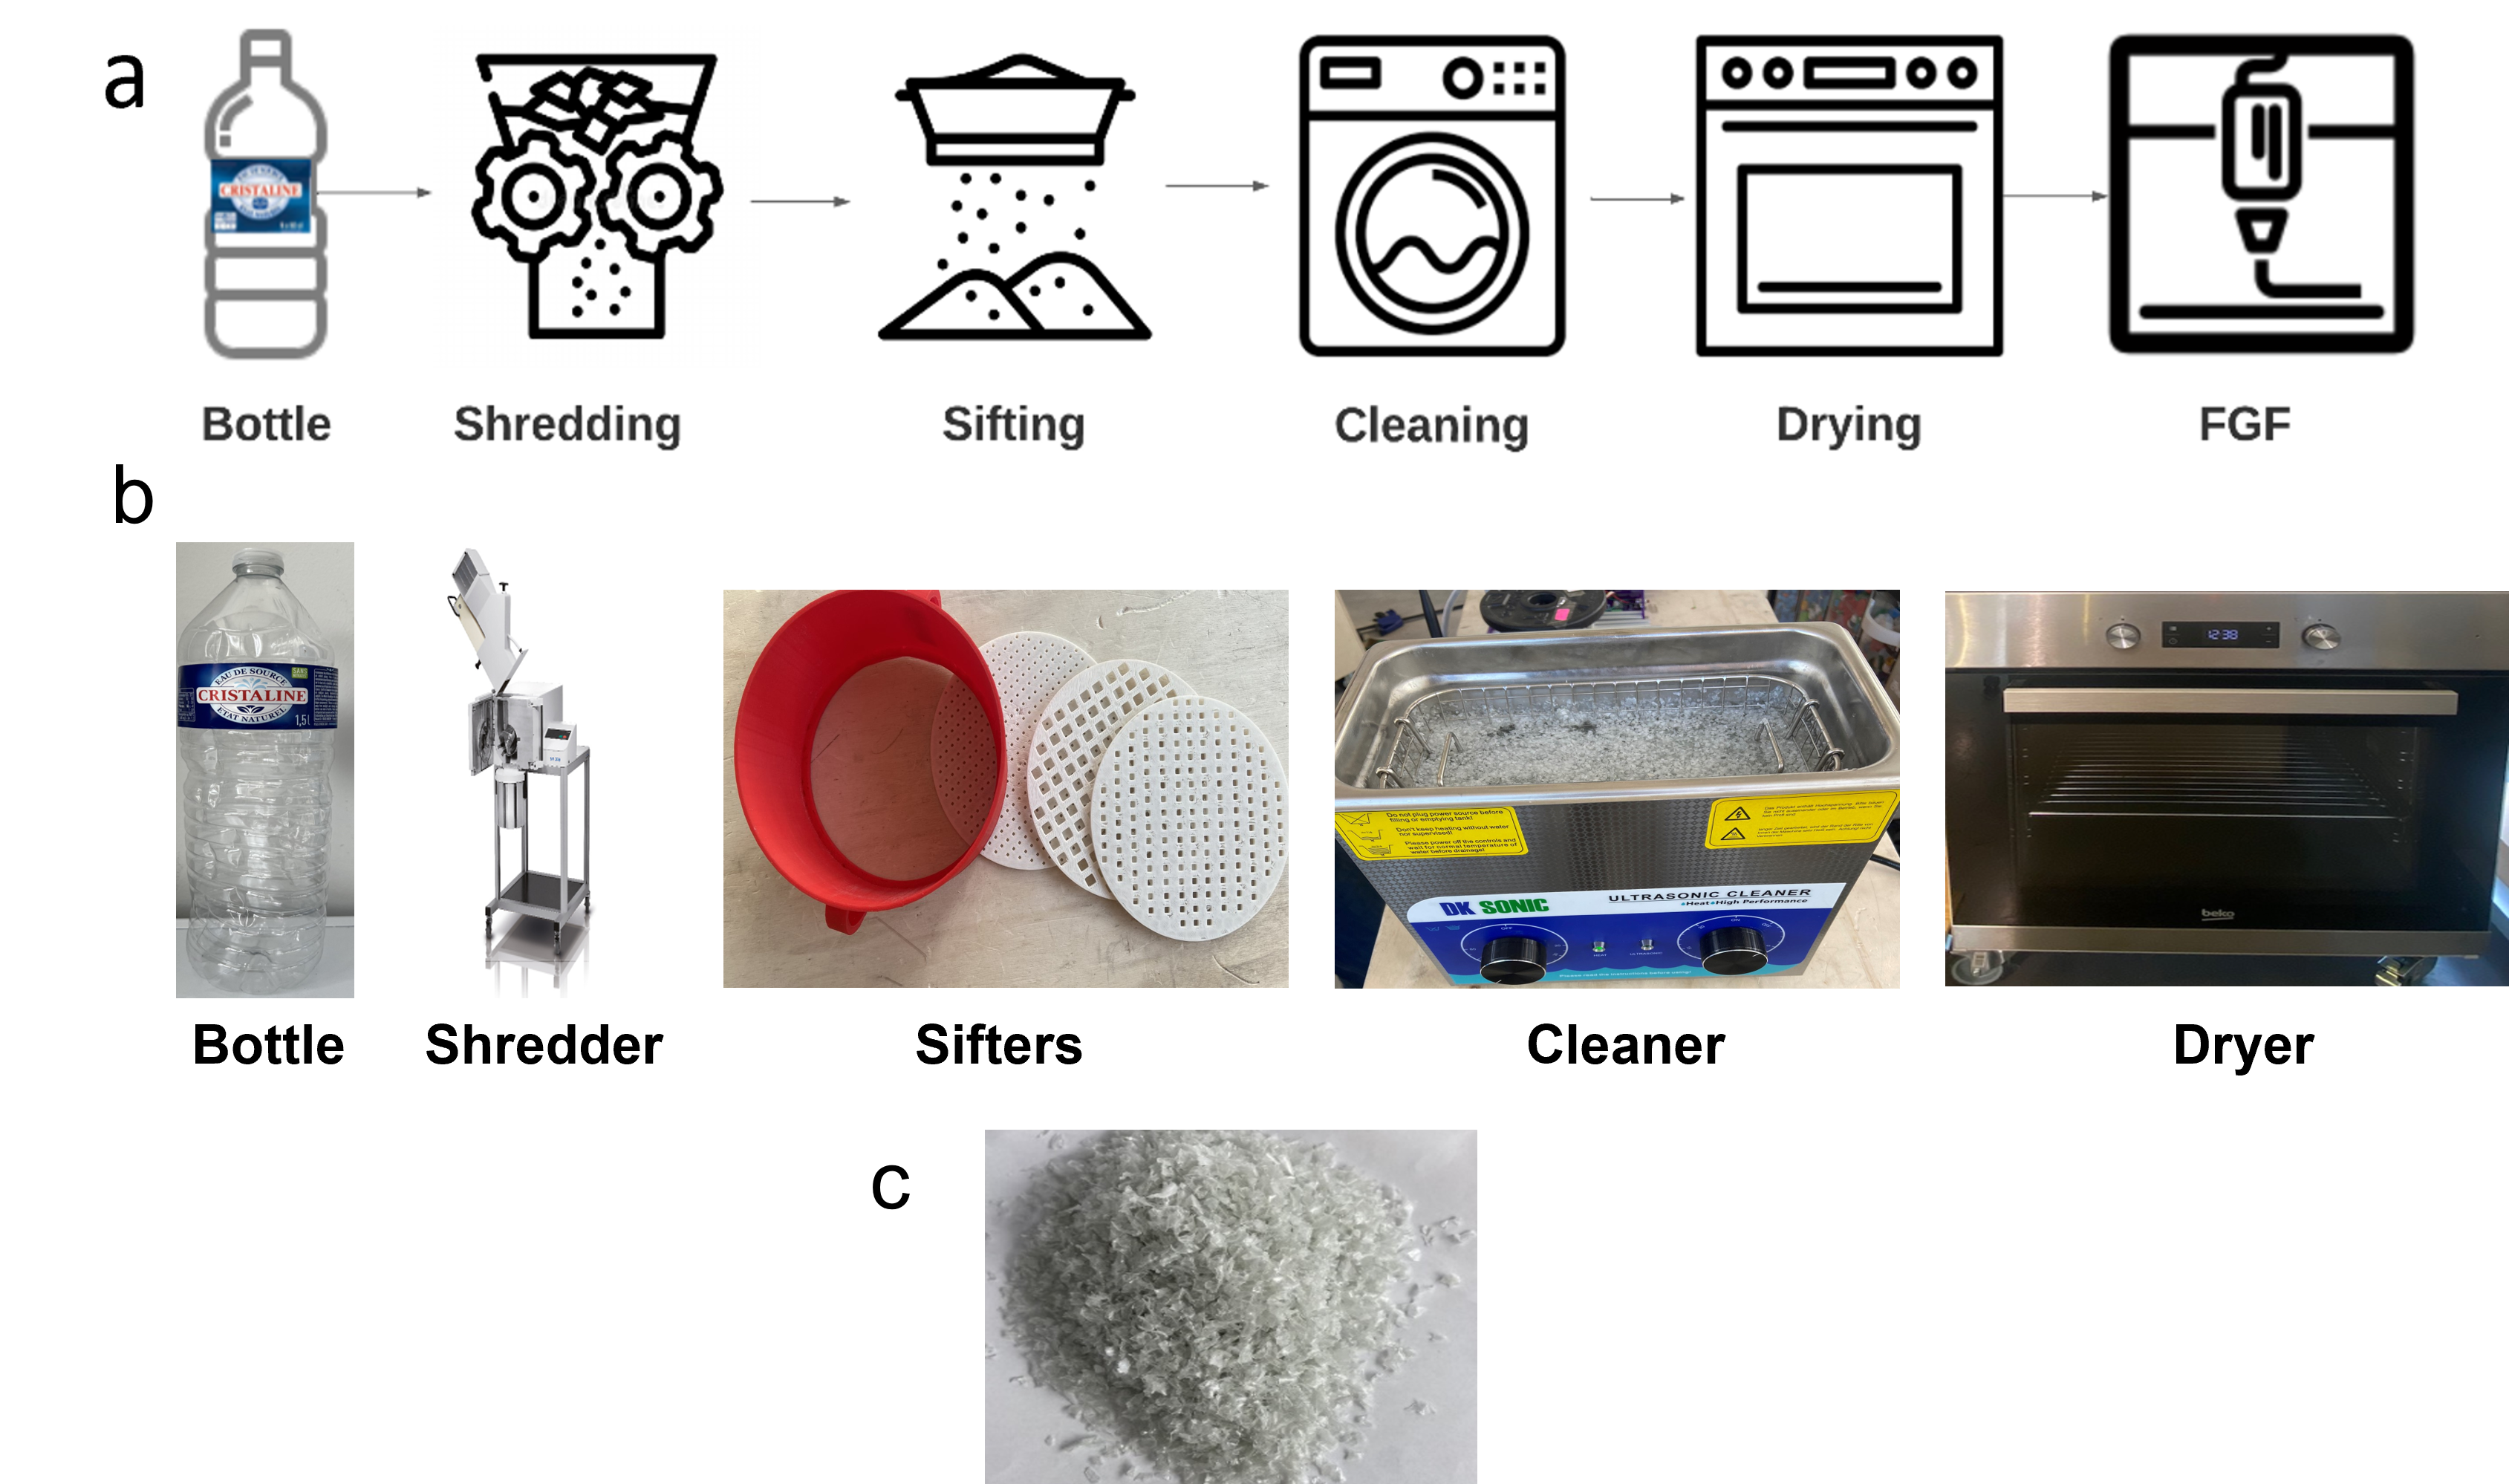
\includegraphics{figures/Fig_2.png}

}

\caption{\label{fig-fig1}Process steps to prepare the collected
material}

\end{figure}

The material composition was calculated as a function of the mass of the
bottles and caps separately. The percent (\%) of bottle-cap was found to
be \textasciitilde90\%rPET (bottle) and \textasciitilde10\% rHDPE (cap).
The complete bottle was shredded without separation of both materials
thus this percentage is constant for all the samples.

\hypertarget{material-preparation-and-characterization}{%
\subsection{Material preparation and
characterization}\label{material-preparation-and-characterization}}

\hypertarget{material-particle-size-analysis--granulometry-}{%
\subsubsection{Material particle size analysis
-Granulometry-}\label{material-particle-size-analysis--granulometry-}}

In order to ensure the particle size suitable for printing, the
characterization of the granulate particles were developed using the
open-source ImageJ software (\protect\hyperlink{ref-imagej2023}{ImageJ,
2023}). The size characteristics of the particles were evaluated between
four different samples; vPET (used as a reference) and the raw material
sifted in three different sizes \(1.5~mm\), \(3~mm\) and \(5~mm\).

\hypertarget{fourier-transform-infrared-spectroscopy-ftir-}{%
\subsubsection{Fourier-transform infrared spectroscopy
--FTIR-}\label{fourier-transform-infrared-spectroscopy-ftir-}}

FTIR spectroscopy was carried out to determine the nature of the bottle
and determine if there were impurities, plasticizers or additives that
could be detected. The analysis were made on samples of rPET and rHDPE
separately and then a printed sample of both materials to determine if
there was possible to observe a chemical bonding. Every sample was
measured in two different points, three times in each point then curves
were normalized and analyzed with the Origin Pro 8. The Fourier
transform infrared spectra have been recorded in the range of
\(4000~cm^{-1}\) to \(375~cm^{-1}\) with resolution \(4~cm^{-1}\) using
Bruker IFS 66V spectrophotometer.

\hypertarget{differential-scanning-calorimetry-dsc-}{%
\subsubsection{Differential scanning calorimetry
--DSC-}\label{differential-scanning-calorimetry-dsc-}}

Differential scanning calorimetry analysis were performed with a DSC-1
Mettler Toledo with STARe software operating under nitrogen atmosphere
at heating rate and cooling rate of \(10~°C/min\). rPET, rHDPE and
rPET90//rHDPE10 samples were investigated using three cycles: first
heating from 20°C to 270 °C, cooling to 20 °C and reheating to 270°C.
The rHDPE sample was analyzed following similar cycles but with the
maximum temperature set at 250°C and the blend with temperatures from
-20 to 270°C. Glass transition temperature (Tg) of rPET was determined
during the first heating cycle, while rPET90//rHDPE10 (Tg) during the
second heating cycle along with the melting point of all materials.
Crystallization temperature (Tc) of the each of the materials was
determined during the cooling cycle. The degree of crystallinity (Xc)
was calculated from the second cycle for recycled materials and first
cycle for the blend as expressed in equation (1)
(\protect\hyperlink{ref-pan2020}{Pan et al., 2020};
\protect\hyperlink{ref-taghavi2018}{Taghavi et al., 2018}):

\begin{equation}\protect\hypertarget{eq-dsc}{}{
X_{c}(\%) = \frac{\Delta H_{m}}{w \cdot \Delta H_{m}^\circ}
}\label{eq-dsc}\end{equation}

Where, \(\Delta H_{m}\) is the latent heat of melt, \(w\) is weight
percentage of polymer in the blend, and \(\Delta H_{m}^\circ\) is the
reference heat of 100\% crystalline PET (\(140~J/g\)) and HDPE
(\(293~J/g\)), respectively, provided in the literature
(\protect\hyperlink{ref-kratofil2006}{Kratofil et al., 2006};
\protect\hyperlink{ref-pan2020}{Pan et al., 2020}).

\hypertarget{melt-flow-index-mfi-}{%
\subsubsection{Melt Flow Index --MFI-}\label{melt-flow-index-mfi-}}

The melt-flow index (MFI) of rPET90//rHDPE10 flakes was determined using
a Instron CEAST MF20. The analysis was performed using three samples of
\textasciitilde5 g at 255 °C using a 2.16 kg weight according to ASTM
D1238. The process was repeated three times. The average value of the
three results was then reported with \(gr/10 \times min\) unit.

\hypertarget{density}{%
\subsubsection{Density}\label{density}}

In order to calculate the material's density, first; the volume was
found measuring the dimensions of a solid \(50x50x50~mm\) cubic geometry
fabricated injecting rPET90//rHDPE10 flakes into a square mould with a
known volume using open-source desktop injection (Holipress, Holimaker,
France) machine. Then the model was weighed, and the mass was obtained.
Finally, density was calculated as expressed in
Equation~\ref{eq-density}. To ensure the accuracy the test was performed
twice and the average value was reported in \(g/cm^{3}\).

\begin{equation}\protect\hypertarget{eq-density}{}{
\rho = V/m    \qquad \left[ \frac{g}{cm^{3}} \right]
}\label{eq-density}\end{equation}

Where, \(\rho\) is the density, \(V\) is the volume, and \(m\) the mass.

Afterwards, experimental results were compared with the theoretical
blend density which could be calculated by
Equation~\ref{eq-density_theory}.

\begin{equation}\protect\hypertarget{eq-density_theory}{}{
\rho_{12}= \frac{1}{\frac{W_{1}}{\rho_{2}} + \frac{W_{2}}{\rho_{2}}} \qquad \left[ \frac{g}{cm^{3}} \right]                                               
}\label{eq-density_theory}\end{equation}

Where, \(\rho_{12}\) is the density of the blend, \(W_{1}\) and
\(W_{2}\), the weight fractions of each polymer, \(\rho_{1}\) and
\(\rho_{2}\), the theoretical density of each polymer for PET
(\(~1.38~g/cm^{3}\)) and HDPE 0.93 to 0.97 \(g/cm^{3}\)
(\protect\hyperlink{ref-jonathanguidigo12017}{Jonathan GUIDIGO1 et al.,
2017}).

\hypertarget{printing-process}{%
\subsection{Printing process}\label{printing-process}}

\hypertarget{establishing-optimal-parameters}{%
\subsubsection{Establishing optimal
parameters}\label{establishing-optimal-parameters}}

Establishing optimum combinations of parameters is essential for better
quality and mechanical properties of the printed parts
(\protect\hyperlink{ref-jaisinghsheoran2020}{Jaisingh Sheoran and Kumar,
2020}). According to Oberloier et al.
(\protect\hyperlink{ref-oberloier2022}{2022a}), particle swarm
optimization (PSO) is an effective and time-effective method for this
purpose. The optimization of the 3-D printing parameters for the
rPET90//rHDPE10 material in the GigabotX was performed using the
open-source PSO Experimenter platform (available in Linux), following
the methodology developed by Oberloier et al.
(\protect\hyperlink{ref-oberloier2022}{2022a}). Three process benchmark
artifacts were printed; line, plane, and cube. They were modeled in CAD
software Onshape CAD v1.150 and sliced using Prusaslicer v2.52.0.
Figure~\ref{fig-cad} presents the geometry models and dimensions.

\begin{figure}

{\centering 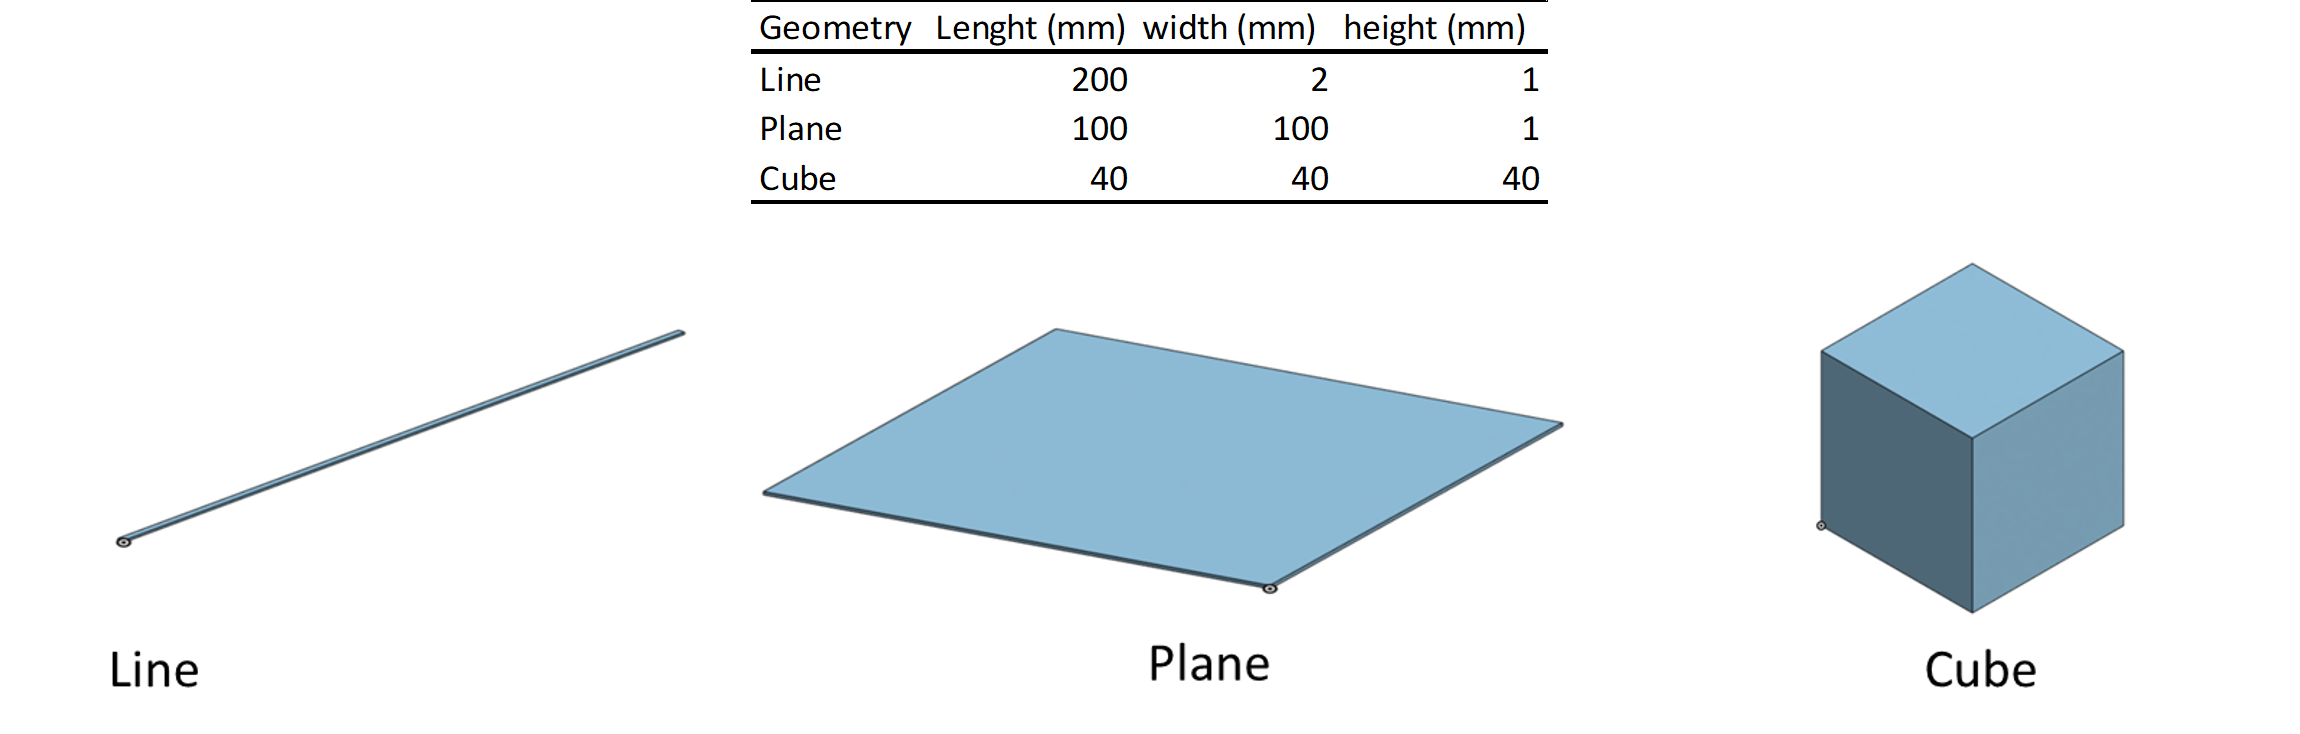
\includegraphics{figures/Figure-2.png}

}

\caption{\label{fig-cad}Dimensions and CAD models of the geometries used
for parameters optimization.}

\end{figure}

Four parameters were assessed: 1) the nozle temperature, 2) bed
temperature, 3) the printing speed and 4) extrusion multiplier
(\protect\hyperlink{ref-oberloier2022a}{Oberloier et al., 2022b}). The
initial parameters for the line are presented in Table 1a while other
parameters were obtained in preliminary experimental work shown in Table
1.b. Finally, the PSO tuning parameters were found in the previous PSO
work (\protect\hyperlink{ref-oberloier2022}{Oberloier et al., 2022a})
Table 1.c.

\begin{table}

\caption{\label{tbl-table1}table 1}\begin{minipage}[t]{\linewidth}
\subcaption{\label{tbl-table1-1}Line optimization initial parameters }

{\centering 

\tabularnewline

\centering\begingroup\fontsize{12}{14}\selectfont

\begin{tabular}{llrrll}
\toprule
Variable & Min & Max & Guess & True/False & Description\\
\midrule
\cellcolor{gray!6}{T1} & \cellcolor{gray!6}{255} & \cellcolor{gray!6}{270} & \cellcolor{gray!6}{260} & \cellcolor{gray!6}{TRUE} & \cellcolor{gray!6}{Temperature Zone 1 on GigabotX}\\
Tb & 80 & 90 & 85 & TRUE & Bed temperature\\
\cellcolor{gray!6}{Ps} & \cellcolor{gray!6}{10} & \cellcolor{gray!6}{25} & \cellcolor{gray!6}{15} & \cellcolor{gray!6}{TRUE} & \cellcolor{gray!6}{Printing Speed}\\
E & 0.5 & 2 & 1 & FALSE & Extrusion Multiplier\\
\bottomrule
\end{tabular}
\endgroup{}

}

\end{minipage}%
\newline
\begin{minipage}[t]{0.50\linewidth}
\subcaption{\label{tbl-table1-2}Fixed parameters to perform printing parameters optimization based on
PSO }

{\centering 

\tabularnewline

\centering\begingroup\fontsize{11}{13}\selectfont

\begin{tabular}{lll}
\toprule
Parameters & Value & Units\\
\midrule
\cellcolor{gray!6}{Layer height} & \cellcolor{gray!6}{0.5} & \cellcolor{gray!6}{mm}\\
Width & 2 & mm\\
\cellcolor{gray!6}{T2} & \cellcolor{gray!6}{230} & \cellcolor{gray!6}{°C}\\
T3 & 220 & °C\\
\cellcolor{gray!6}{Cooling} & \cellcolor{gray!6}{0} & \cellcolor{gray!6}{\%}\\
\addlinespace
Infill density & 2 & \%\\
\bottomrule
\end{tabular}
\endgroup{}

}

\end{minipage}%
%
\begin{minipage}[t]{0.05\linewidth}

{\centering 

~

}

\end{minipage}%
%
\begin{minipage}[t]{0.45\linewidth}
\subcaption{\label{tbl-table1-3}Recommended parameters for PSO tuning }

{\centering 

\tabularnewline

\centering\begingroup\fontsize{11}{13}\selectfont

\begin{tabular}{lr>{\raggedright\arraybackslash}p{4cm}}
\toprule
Variable & Value & Description\\
\midrule
\cellcolor{gray!6}{Kv} & \cellcolor{gray!6}{0.5} & \cellcolor{gray!6}{The emphasis given to the velocity component}\\
Kp & 1.0 & The emphasis given to a particle's personal best position\\
\cellcolor{gray!6}{Kg} & \cellcolor{gray!6}{2.0} & \cellcolor{gray!6}{The emphasis given to the swarm's group best position}\\
\bottomrule
\end{tabular}
\endgroup{}

}

\end{minipage}%

\end{table}

\hypertarget{fused-granular-fabrication-fgf-}{%
\subsubsection{Fused Granular Fabrication
--FGF-}\label{fused-granular-fabrication-fgf-}}

To print the raw material obtained, a 3-heat-zone modified open-source
printer (Gigabot XL re:3D, Houston, TX, USA) was used as illustrated in
Figure~\ref{fig-gigabot}. The machine is a single screw extrusion-based
3-D printer capable of direct printing pellets, flakes or granules, with
a nozzle size of \(1.75~mm\). For this study, a chair was printed to
evaluate the ability for the material to 3-D print and the machine
capacity to print large-objects such as a piece of furniture. The ideal
parameters found for the cube geometry were used to print the final
part.

\begin{figure}

{\centering 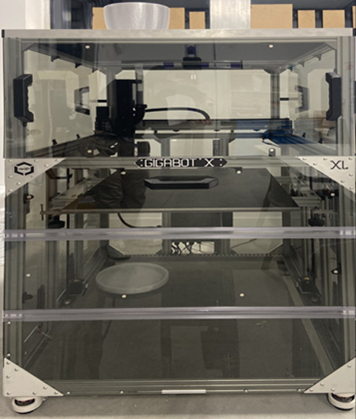
\includegraphics{figures/Figure_4_Giga.png}

}

\caption{\label{fig-gigabot}Fused granular fabrication printer Gigabot}

\end{figure}

\hypertarget{results-and-discussion}{%
\section{Results and discussion}\label{results-and-discussion}}

\hypertarget{material-characterization}{%
\subsection{Material characterization}\label{material-characterization}}

Both polymeric components of the bottle as well as the blend were
characterized and analyzed to determine their properties using different
methods as explained in the previous section.

\hypertarget{material-particle-size-analysis-granulometry}{%
\subsubsection{Material particle size analysis
(granulometry)}\label{material-particle-size-analysis-granulometry}}

Previous studies demonstrated that particles with areas smaller than
\(22~mm^{2}\) were optimal for print without jamming or under-extrusion
problems (\protect\hyperlink{ref-woern2018}{Woern et al., 2018}). From
the experiments conducted, however, particles with areas above
\(10~mm^{2}\) clogged in the feeding system and auger screw of the
machine. Therefore, granulometry analysis was performed using three
different mesh sizes.

\begin{figure}

\begin{minipage}[t]{0.57\linewidth}

{\centering 

\raisebox{-\height}{

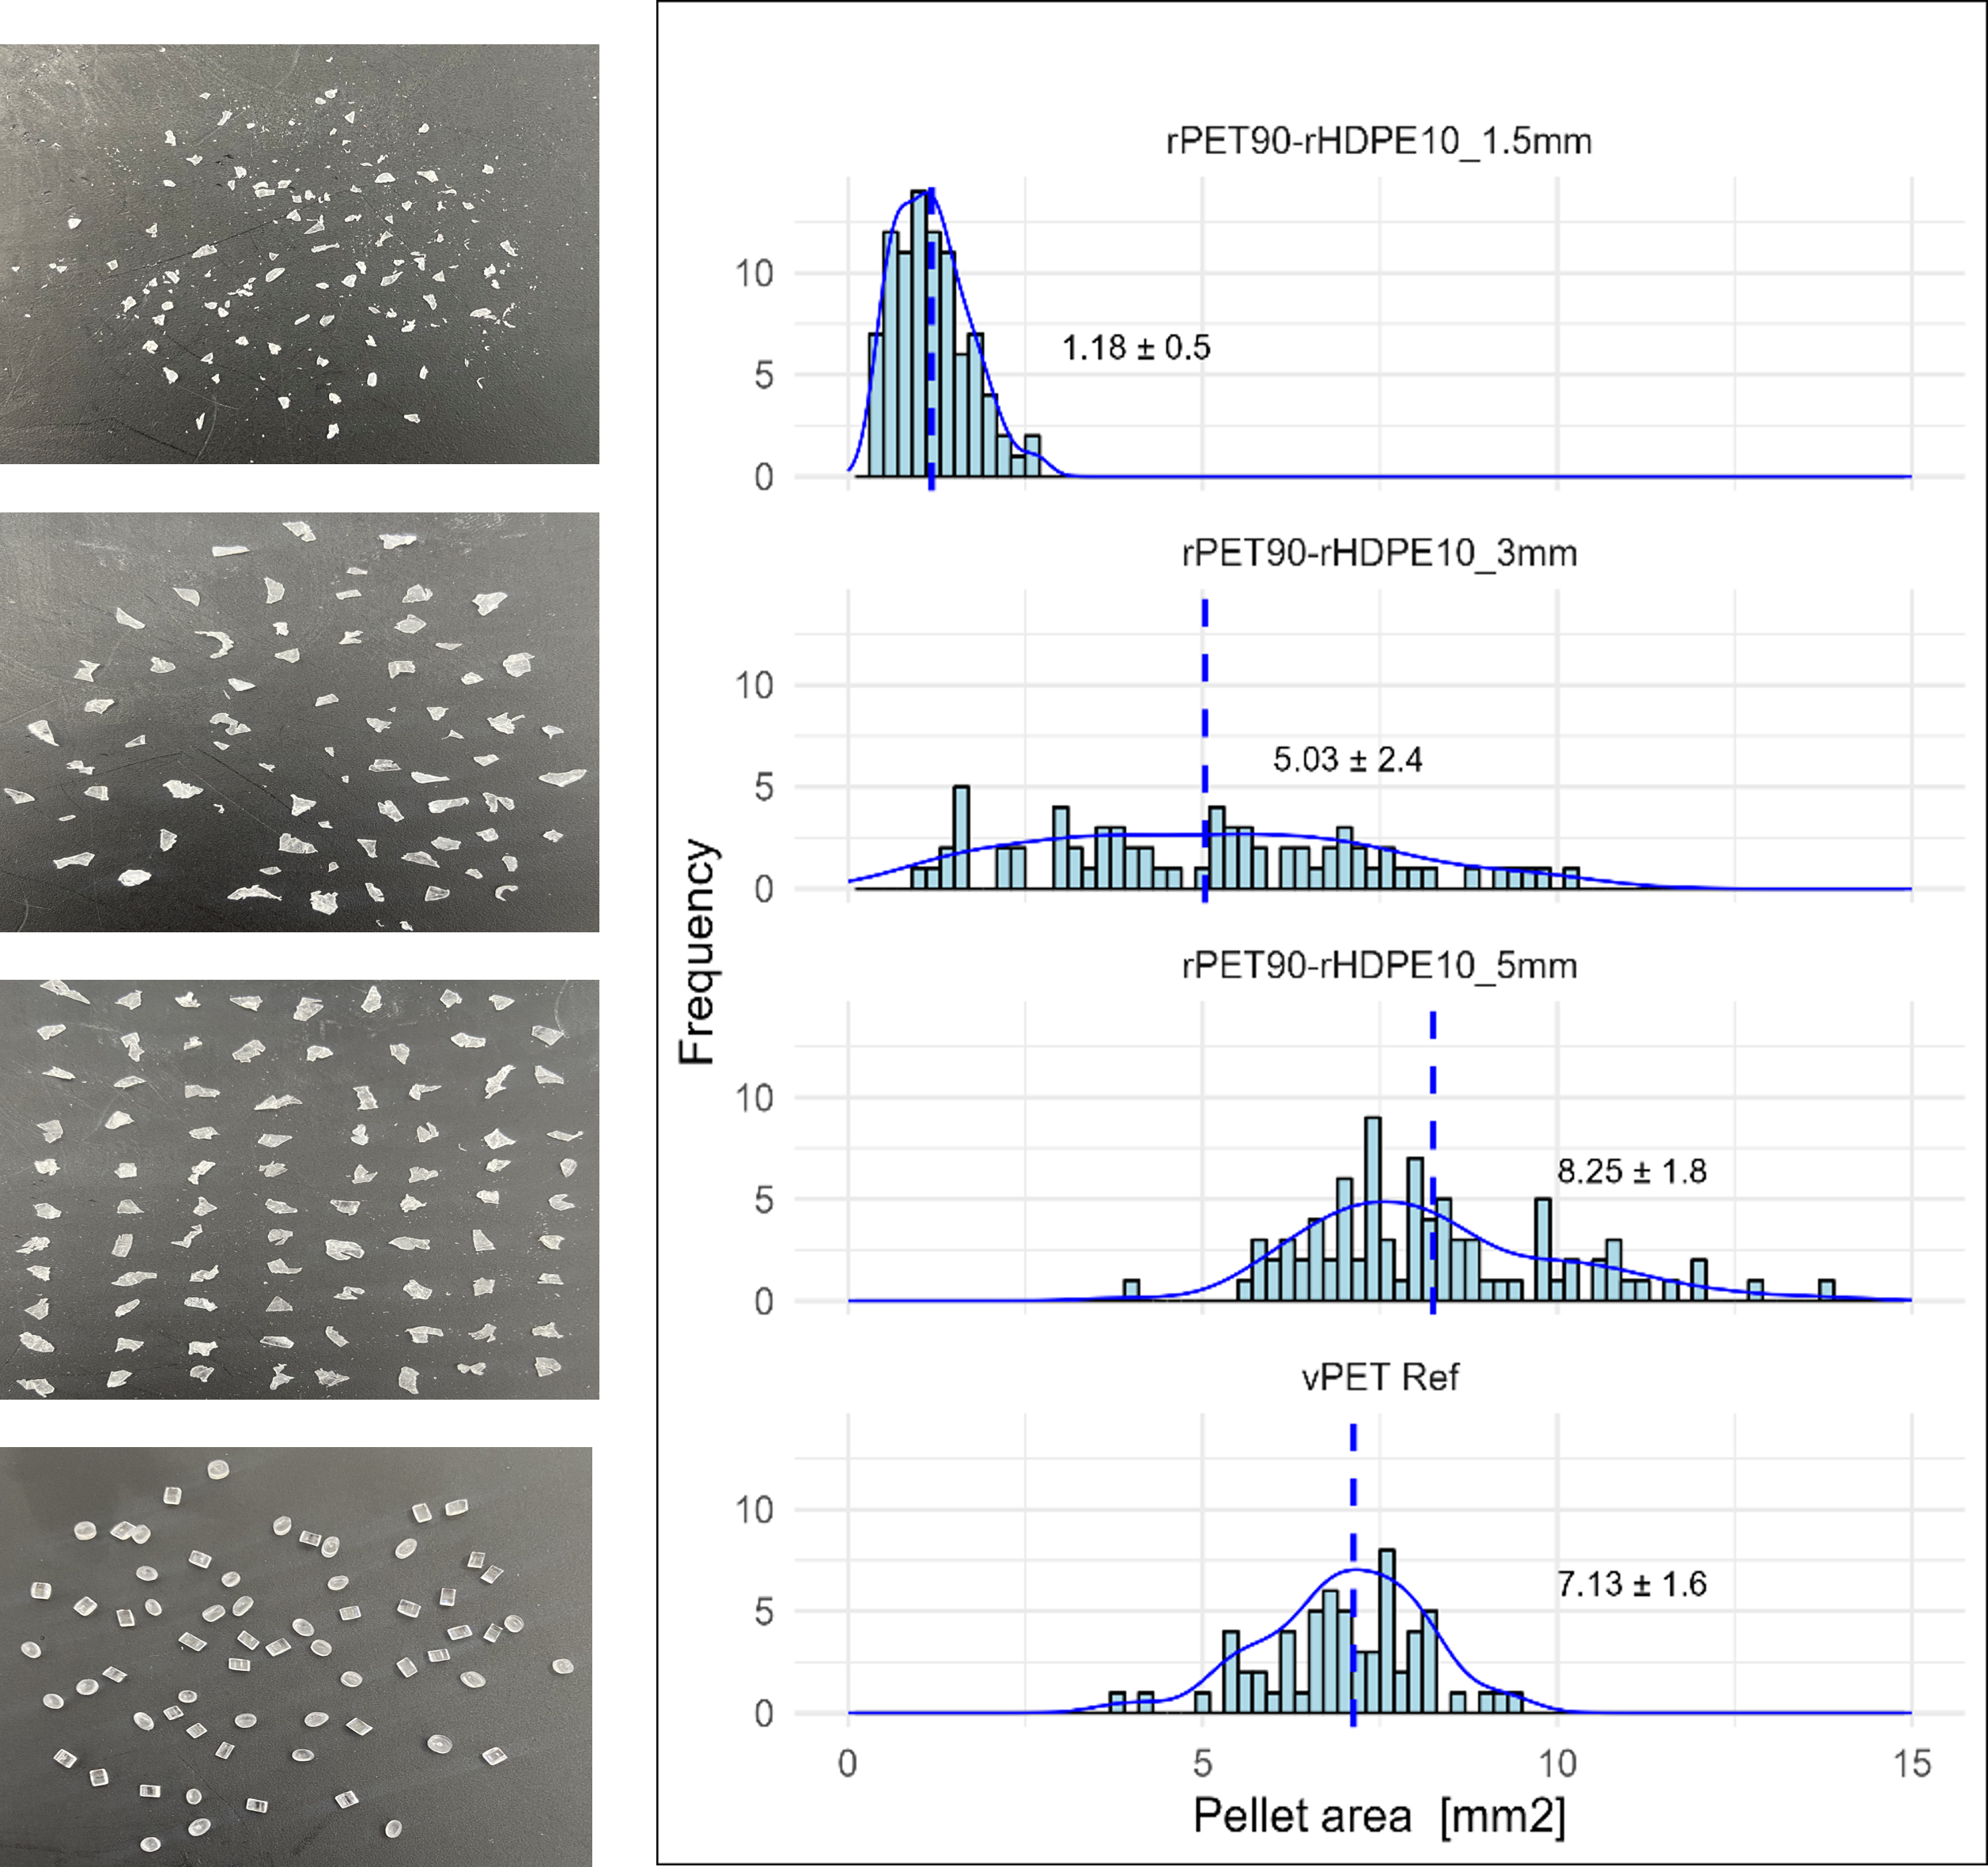
\includegraphics{figures/Figure_5_granulometry.png}

}

\caption{\label{fig-granulometry}Granulometry analysis}

}

\end{minipage}%
%
\begin{minipage}[t]{0.03\linewidth}

{\centering 

~

}

\end{minipage}%
%
\begin{minipage}[t]{0.40\linewidth}

{\centering 

\raisebox{-\height}{

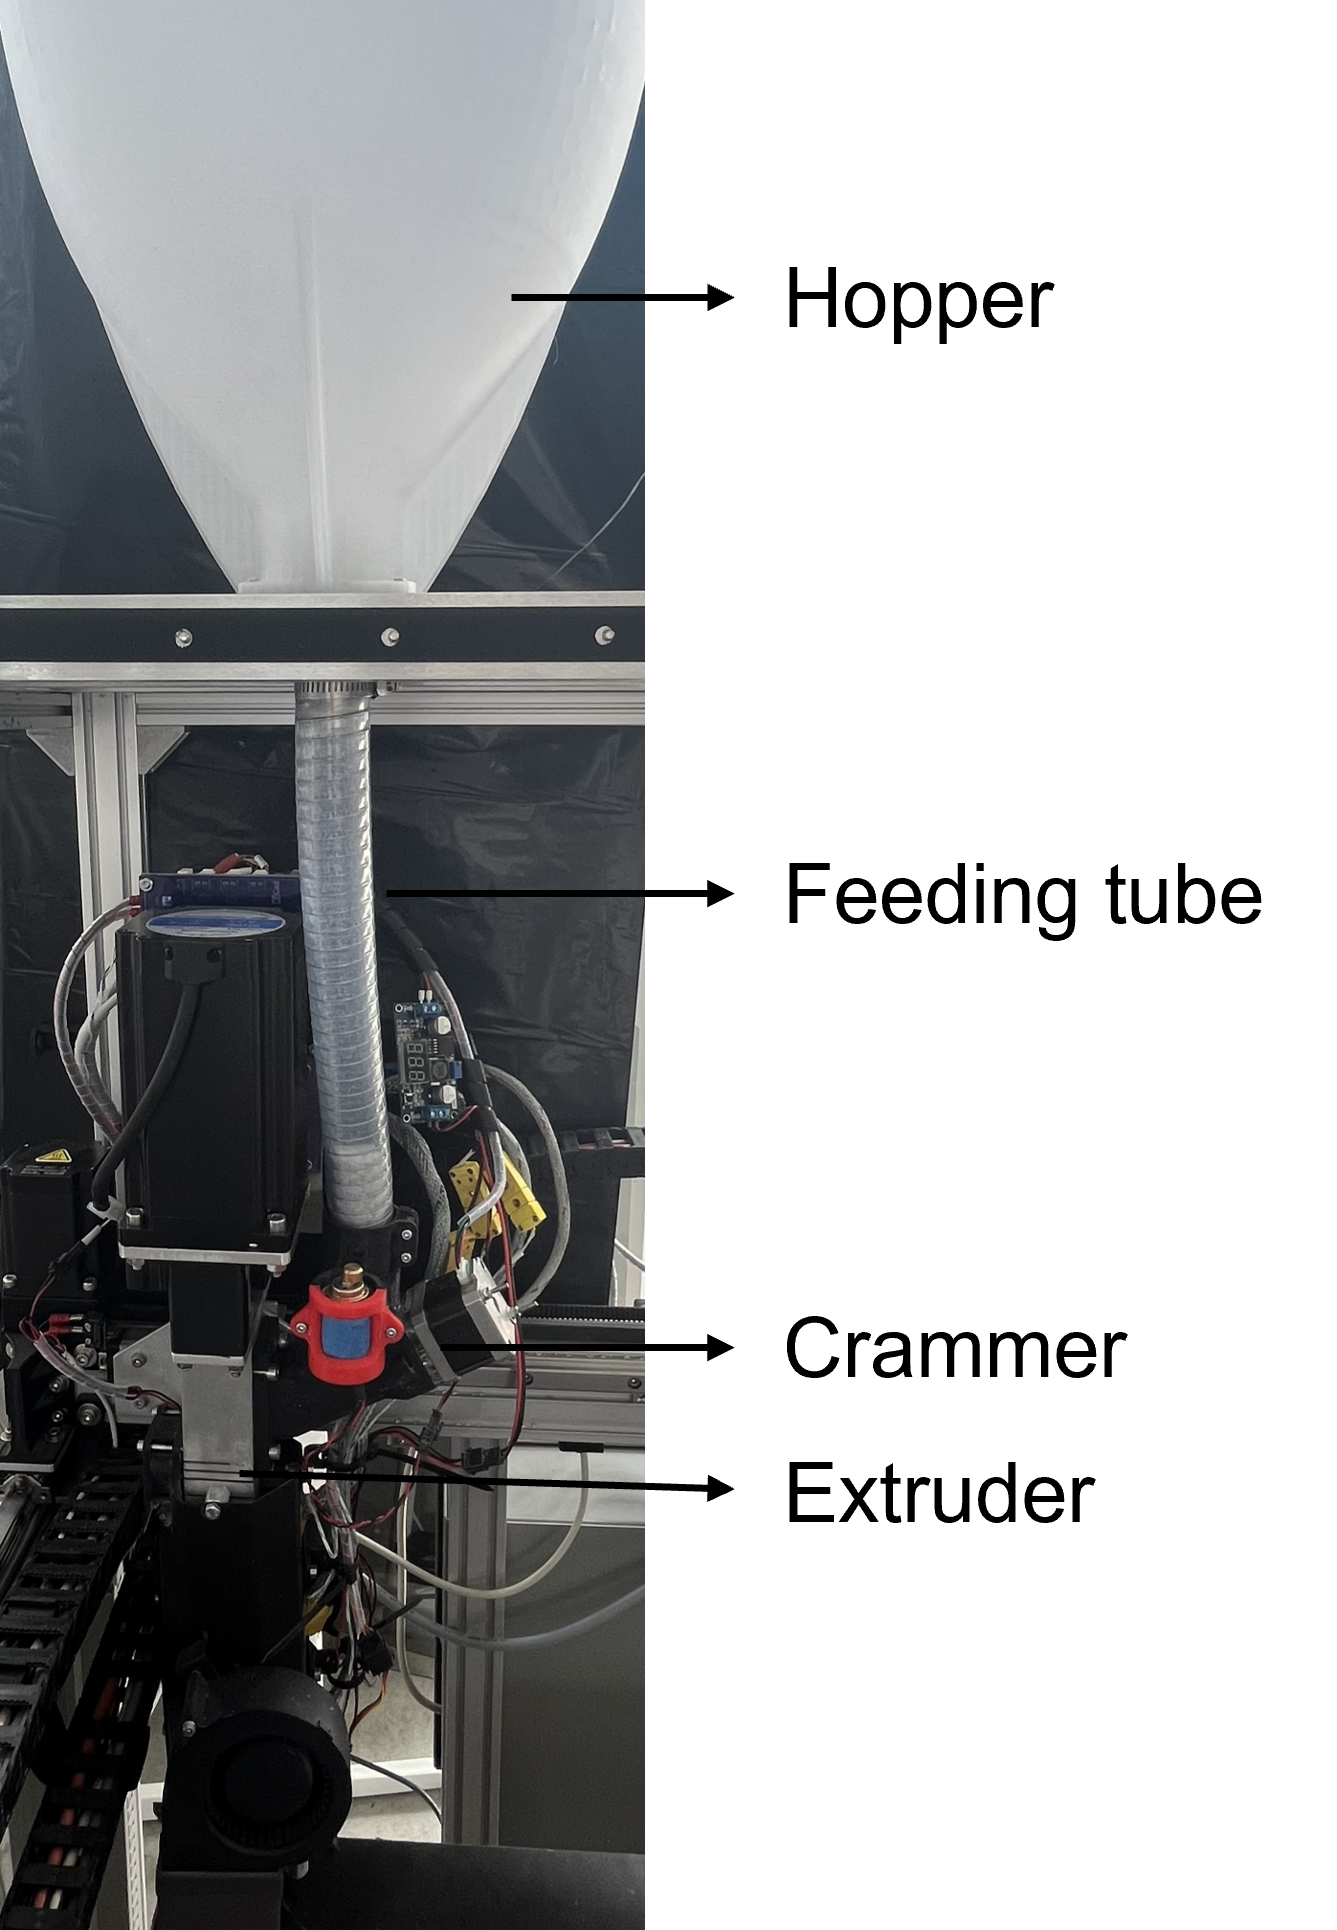
\includegraphics{figures/Figure_6_crammer.png}

}

\caption{\label{fig-crammer}Gigabot feeding system}

}

\end{minipage}%

\end{figure}

Figure~\ref{fig-granulometry} shows the results obtained, where
particles sifted at \(5~mm\) had an average area similar to the
reference. There are, however, particles with areas over \(9~mm^{2}\)
which blocked in the feeding and extrusion section. Particles sifted to
\(1.5~mm\) showed a distribution with areas from 0 to proximately
\(3~mm^{2}\), this area was considered too low for printing. Small
particles can completely melt in the first heat zone obstructing the
consistent flow of other particles and not allowing the pressure needed
to extrude the melted particles lower in the screw. Although flakes of 3
mm show a more dispersed distribution and slightly lower area compared
with the reference, those particles were found to be optimal for
printing.

The final objects, however, still displayed under-extrusion issues. For
this reason, a crammer was implemented
(\protect\hyperlink{ref-little2020}{Little et al., 2020}) as presented
in Figure~\ref{fig-crammer}; which physically pushes particles to the
auger to convey them from feeding tube into the extruder. After the
crammer implementation under-extrusion issues were significatively
decreased. It was concluded that flakes with areas between
\(1.5~mm^{2}\) to \(10~mm^{2}\) were optimum for print using a crammer
able to aid the feeding system.

\hypertarget{chemical-analysis-from-ftir}{%
\subsubsection{Chemical analysis from
FTIR}\label{chemical-analysis-from-ftir}}

Chemical structure information of the materials was obtained using FTIR
spectroscopy, which provided analysis of the characteristic spectral
bands of the polymers.

First, for the rPET (bottle) four characteristic bands can be observed
Figure~\ref{fig-FTIR}, one in \(1713 cm^{-1}\) representing the \(C=O\)
double bond, the \(C-O\) single bond ester at \(1240 cm^{-1}\),
\(1093 cm^{-1}\) band corresponding to the methylene group and
vibrations of the ester bond and finally, a band \(722 cm^{-1}\) the CH2
rocking bending vibration.

Similar results were obtained in the literature for PET coming from
recycled water bottles, soda bottles and food containers
(\protect\hyperlink{ref-zander2018}{Zander et al., 2018}). For rHDPE
(caps), four characteristic peaks were observed, the bond of C-H
functional group in peaks \(2915cm^{-1}\) and \(2847~cm^{-1}\), main
bending mode of the -CH2 in \(1465~cm^{-1}\) and CH2 rocking bending
vibration at \(729 ~cm^{-1}\). These results confirmed the chemical
structures of starting materials. Additionally, other indicative
resonances besides those associated with the polymer structures were not
observed, concluding that additives or plasticizers in significative
quantities were not present in either sample. The spectrum of the
printed blend (rPET90//rHDPE10) had the same characteristic peaks as the
bottle, confirming the PET dominant content. There are, however,
observable differences between \(1000 ~cm^{-1}\) and \(720 ~cm^{-1}\)
and in the bond of C-H (\(2915~cm^{-1}\) and \(2847 ~cm^{-1}\) peaks),
confirming the presence of HDPE (cap). The shifting observed can be
attributed to interactions between both materials.

\begin{figure}

{\centering 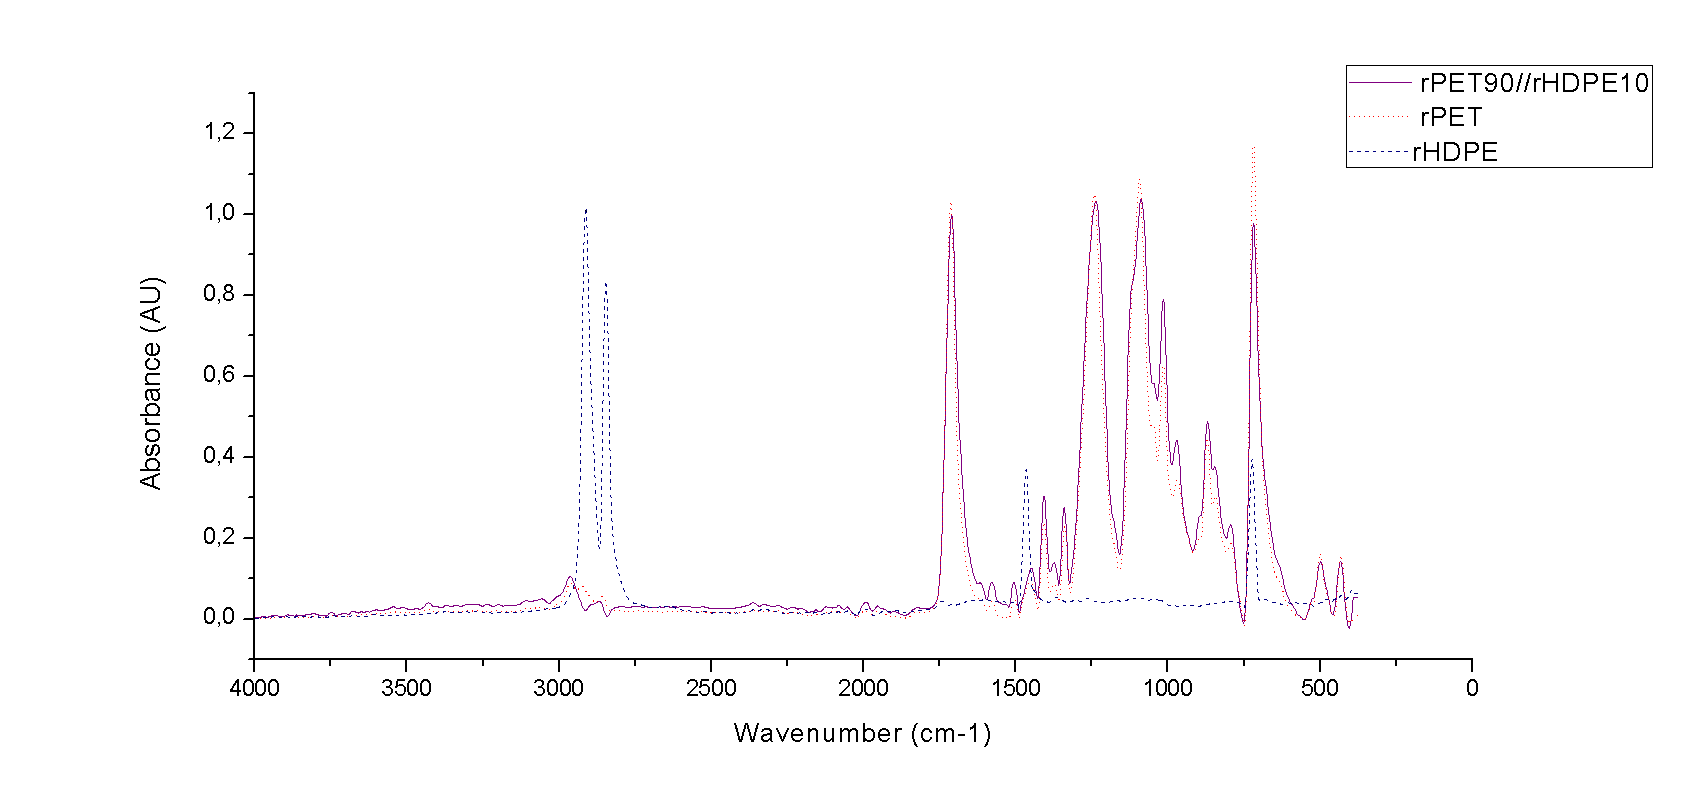
\includegraphics[width=0.9\textwidth,height=\textheight]{figures/Figure_7_FTIR.png}

}

\caption{\label{fig-FTIR}FTIR spectra of rPET, rHDPE and their blend}

\end{figure}

\hypertarget{thermal-analysis-dsc}{%
\subsubsection{Thermal analysis DSC}\label{thermal-analysis-dsc}}

The thermal properties of both recycled materials and their blend were
characterized via DSC to have a starting point for the 3-D printing
process parameter optimization.

From the representative heating and cooling thermograms shown in
Figure~\ref{fig-DCS}, two distinct endothermic peaks are observed in the
printed blend sample that are associated with fusion of the crystalline
fractions of rHDPE and rPET, which confirms the immiscibility of both
materials. Moreover, a significant reduction in the enthalpy of fusion
and crystallization of the rHDPE in the blend is attributed to the low
percentage of HDPE in the blend. The observation of cold crystallization
peak in the blend but not in the individual polymers, however, can be
attributed to an interaction between both polymers, where the rHDPE
might act as a nucleating agent. Table 2. list the thermal properties
for rPET, rHDPE and rPET90//rHDPE10. The melting point for rHDPE and
rPET are 131.7 °C and 249.9 °C, respectively and are similar to those
found in the literature (\protect\hyperlink{ref-chen2015}{Chen et al.,
2015}; \protect\hyperlink{ref-lei2009}{Lei et al., 2009};
\protect\hyperlink{ref-vaucher2022}{Vaucher et al., 2022}). It is
observed that the melting and crystallization temperature of rPET
shifted to a higher value, while slightly decreasing for rHDPE. In
addition, the crystallization of rPET was found be somewhat affected by
the addition of rHDPE as it was increased 4\%. It is likely that the
addition of the rHDPE acted as germination point for crystallization
(\protect\hyperlink{ref-vaucher2022}{Vaucher et al., 2022}). The slight
changes in the rPET temperatures of fusion-crystallization and degree of
crystallinity showed the interaction of both polymers.

\begin{figure}

\begin{minipage}[t]{\linewidth}

{\centering 

\raisebox{-\height}{

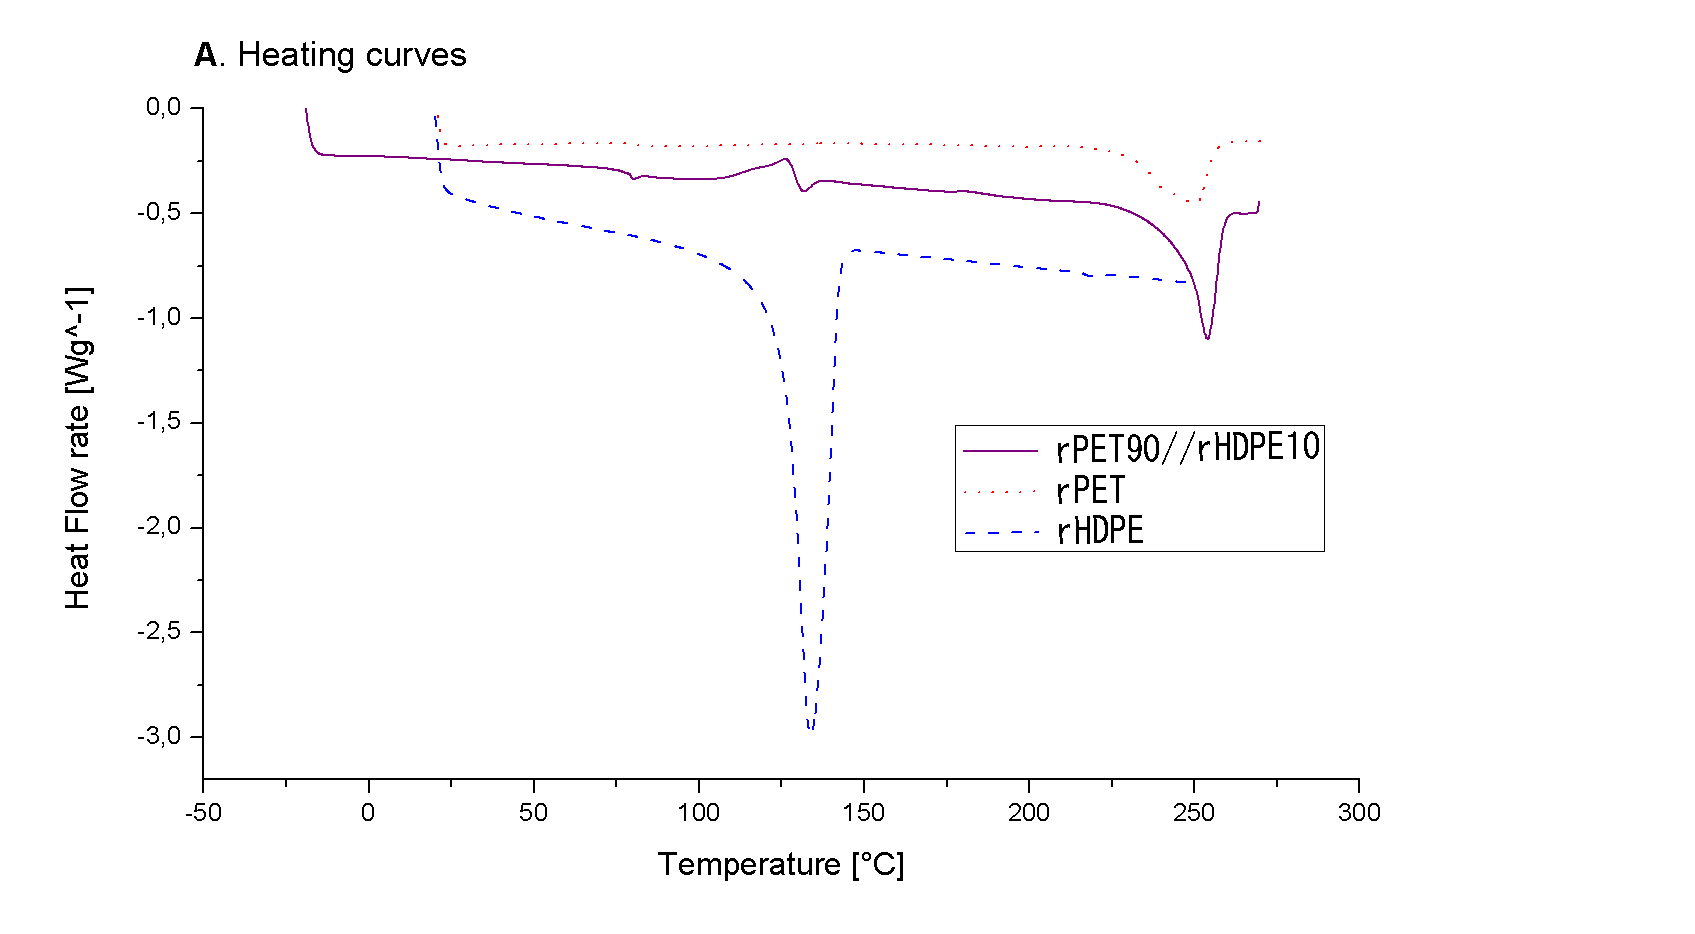
\includegraphics{figures/Figure_8a_DSC.png}

}

}

\subcaption{\label{fig-DCSa}Heating curves}
\end{minipage}%
\newline
\begin{minipage}[t]{\linewidth}

{\centering 

\raisebox{-\height}{

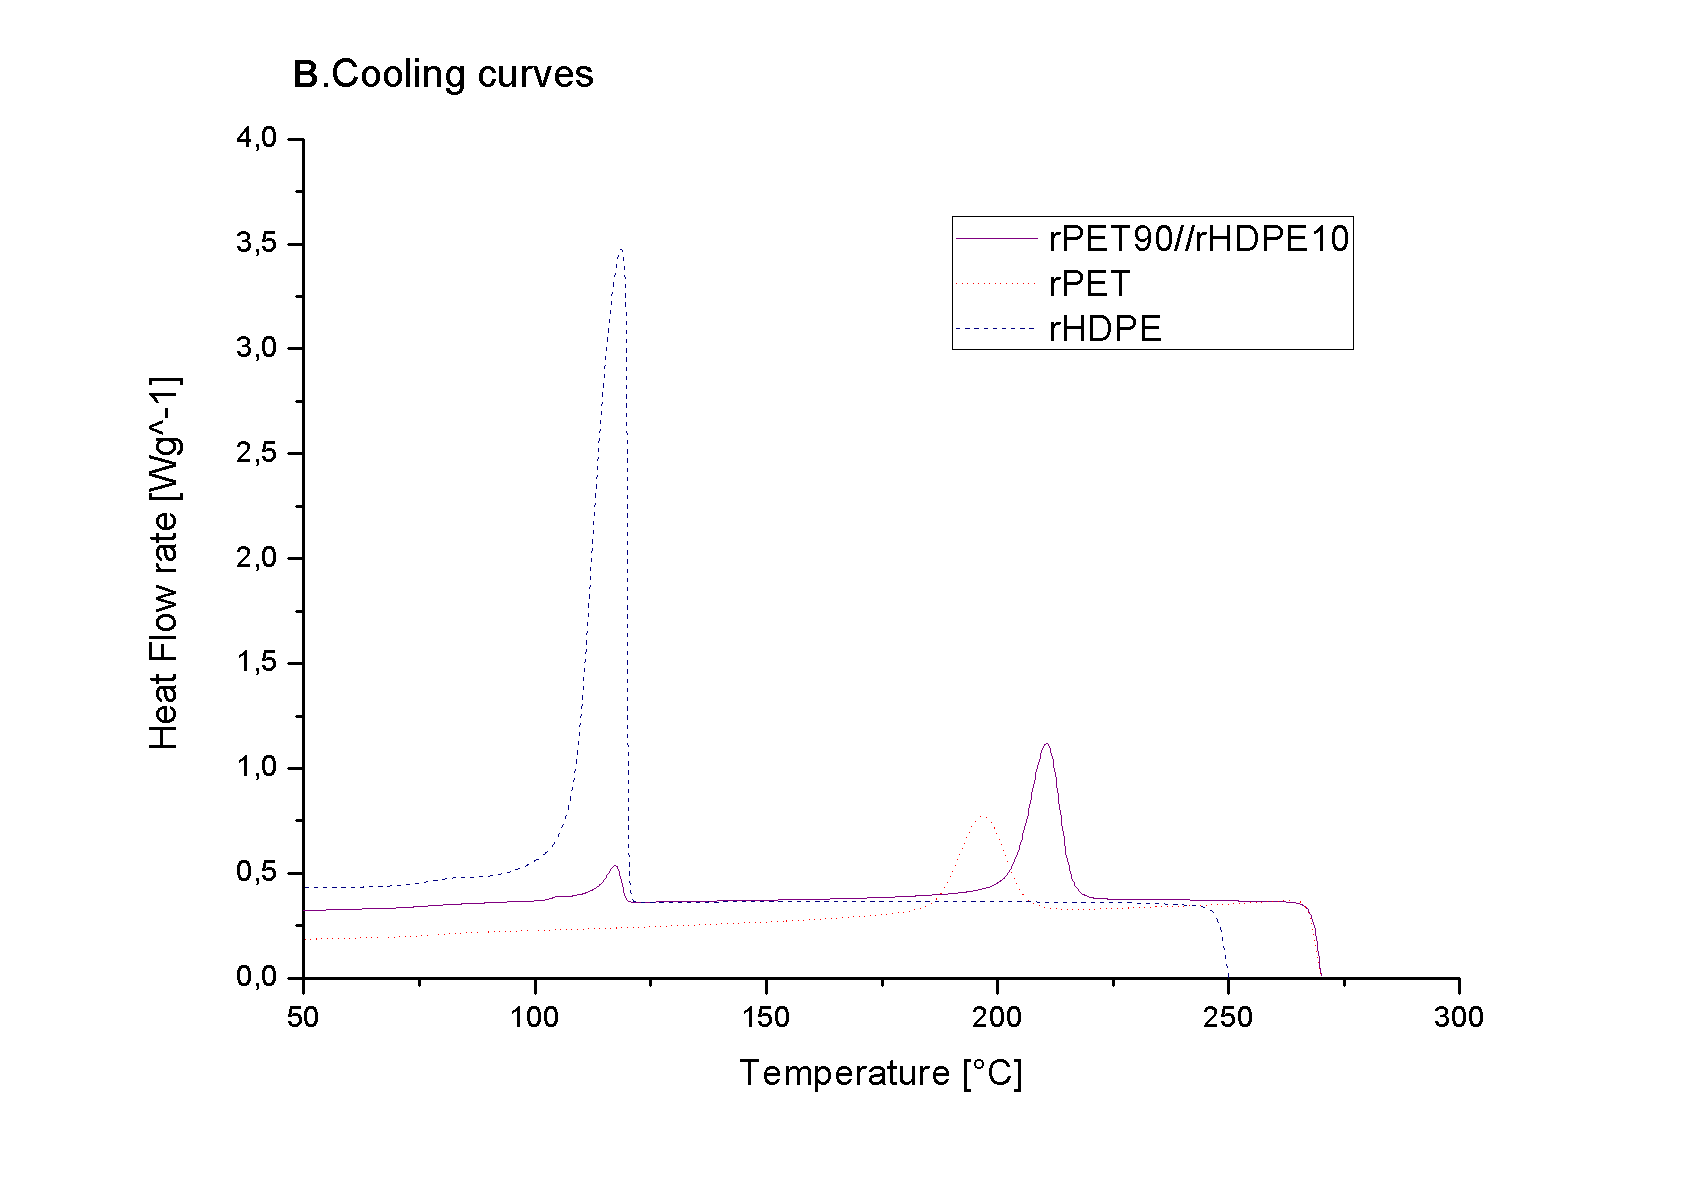
\includegraphics{figures/Figure_8b_DSC.png}

}

}

\subcaption{\label{fig-DCSb}Cooling curve}
\end{minipage}%

\caption{\label{fig-DCS}DSC thermograms of recycled materials and
blends}

\end{figure}

\begin{table}
\caption{Thermal analysis of rPET, rHDPE and their blend}\tabularnewline

\centering\begingroup\fontsize{8}{10}\selectfont

\begin{tabular}[t]{llllllll}
\toprule
\multicolumn{1}{c}{ } & \multicolumn{1}{c}{Glass transition} & \multicolumn{2}{c}{Melting} & \multicolumn{3}{c}{Crystallization } & \multicolumn{1}{c}{\% Crystallinity} \\
\cmidrule(l{3pt}r{3pt}){2-2} \cmidrule(l{3pt}r{3pt}){3-4} \cmidrule(l{3pt}r{3pt}){5-7} \cmidrule(l{3pt}r{3pt}){8-8}
Sample & Tg (°C) & Tm  (°C ) & ΔHm (J/g) & Tc  (°C ) & ΔHc (J/g) & ΔHcc (J/g) & Xc\\
\midrule
\cellcolor{gray!6}{rPET} & \cellcolor{gray!6}{82} & \cellcolor{gray!6}{249.9} & \cellcolor{gray!6}{31.6} & \cellcolor{gray!6}{196.7} & \cellcolor{gray!6}{34.8} & \cellcolor{gray!6}{-} & \cellcolor{gray!6}{22.6}\\
rHDPE & - & 133.8 & 172 & 118.7 & 158.5 & - & 58.7\\
\cellcolor{gray!6}{rPET90/rHDPE10} & \cellcolor{gray!6}{77 / -} & \cellcolor{gray!6}{254/131.7} & \cellcolor{gray!6}{40.3/1.30} & \cellcolor{gray!6}{210.6/117.4} & \cellcolor{gray!6}{37.9/6.7} & \cellcolor{gray!6}{6.8} & \cellcolor{gray!6}{24.8 / 18.4}\\
\bottomrule
\end{tabular}
\endgroup{}
\end{table}

\hypertarget{rheology-mfi}{%
\subsubsection{Rheology MFI}\label{rheology-mfi}}

The melt flow index of the flakes was determined, enabling a fast and
practical screening of the viscosity of the material. Following the DSC
results, the initial temperature to start the MFI test was 250°C,
however the material did not flow reliably so the temperature was
increased by 5°C to enable the melt flow index of the rPET90//rHDPE10 to
be determined. A temperature of 260°C was also tested, however, the
material flowed rapidly and the measurement could not be reliably
obtained. MFI tests were performed three times and the results of the
rPET90//rHDPE10 was a medium MFI 39.4± 2.4 g/10min, which is roughly
consistent with values found in literature for rPET
(\protect\hyperlink{ref-bustosseibert2022}{Bustos Seibert et al., 2022};
\protect\hyperlink{ref-Langer2020}{Langer et al., 2020};
\protect\hyperlink{ref-nofar2019}{Nofar and Oğuz, 2019}). This result
suggests that the low percentage addition of HDPE do not highly impact
the MFI value of rPET. As the material flowed at temperature of 255°C in
the MFI, it provided the input temperature for 3-D printer parameters
optimization.

\hypertarget{density-1}{%
\subsubsection{Density}\label{density-1}}

The density allows the estimation of cost, material use, time consumed
and weight of the printing object in the slicer. This information is
useful to find the accurate printing parameters with the PSO
experimenter as fitness is calculated as a function of the dimensional
accuracy and weight of the printed object. Hence, density was useful to
determine the weight of the geometries.

From calculations made after weight and measuring the rPET90//rHDPE10
injected object, the density of the material was found to be 1.13
\(g/cm^{3}\). The inclusion of HDPE in the matrix polymer led to a
slight decrease in its density, which is a common outcome when a polymer
is mixed with a lower density polymer. However, if we consider a
PET/HDPE blend with a mass ratio of 90/10, the calculated theoretical
density is 1.32 \(g/cm^{3}\). The observed decrease of 14\% in the
results could be attributed to factors such as experimental conditions
and manual measurements.

\hypertarget{particle-swarm-optimization-pso-experimenter}{%
\subsection{Particle swarm optimization (PSO)
Experimenter}\label{particle-swarm-optimization-pso-experimenter}}

Geometries were 3-D printed changing the parameters as expressed in the
PSO Experimenter software. The fitness function is defined by the
weighted sum of the dimensional measurements (length, width, height, and
weight) of the printed object, where fitness below 0.1 was set as a
desirable threshold. In the software five particles were established for
one iteration, thus in one iteration five different parameters
combinations were printed. The first geometry (line) was able to reach a
fitness of \textless{} 0.1 after six iterations for a total of thirty
lines printed. The ideal parameters for this geometry are listed in
column two of Table~\ref{tbl-table3} and images of the resulting
geometries are illustrated in Figure~\ref{fig-geometries} .

\begin{figure}

{\centering 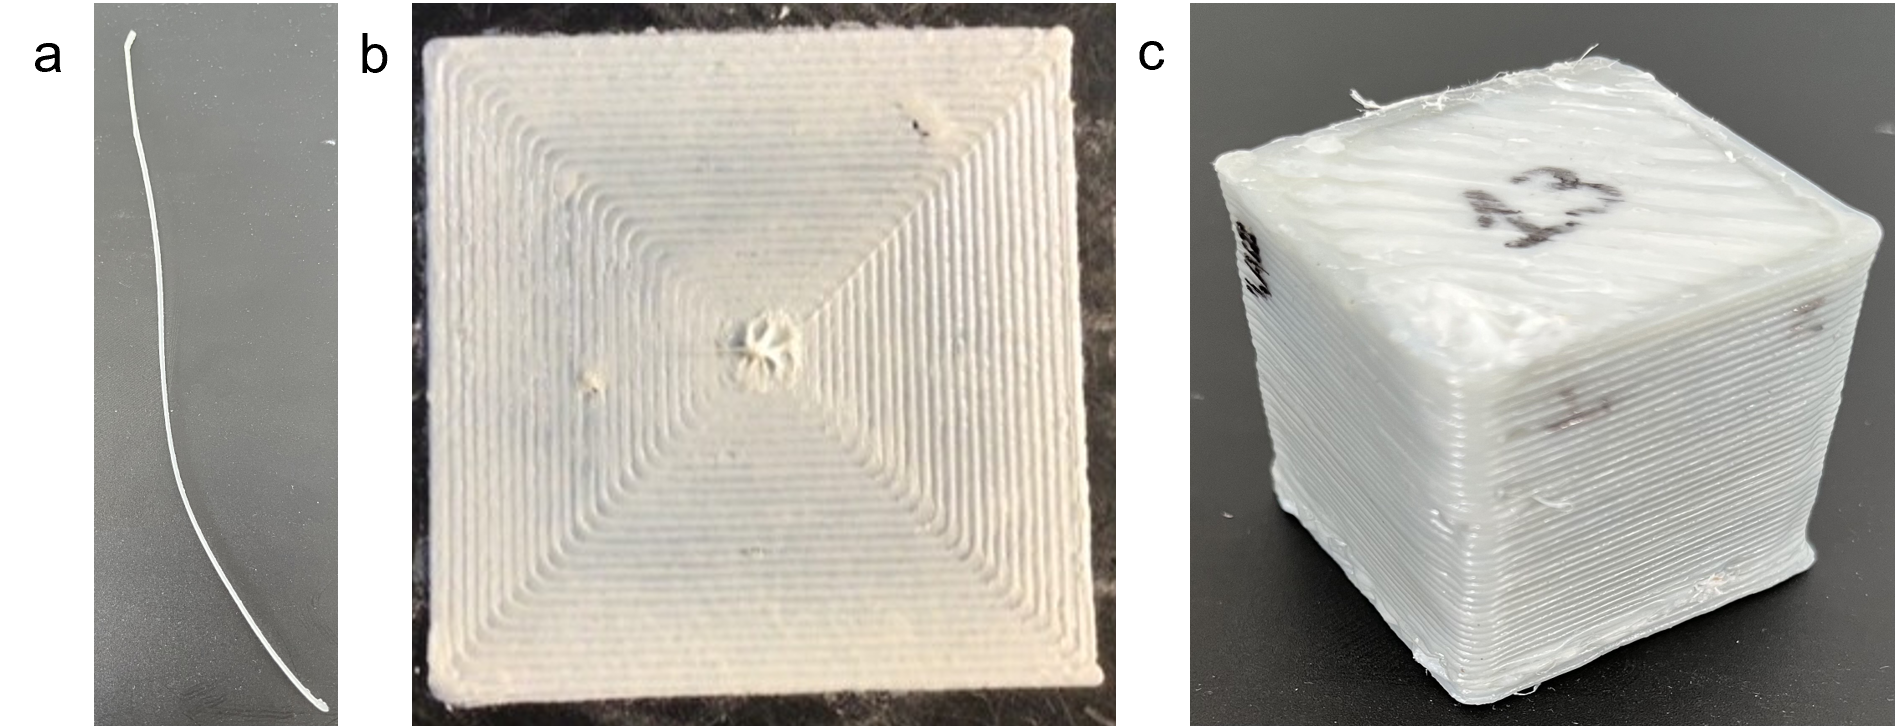
\includegraphics{figures/Figure_9_geometries.png}

}

\caption{\label{fig-geometries}Images of the resulting geometries a)
line, b) plane, c) cube}

\end{figure}

Afterwards, these parameters were used as initial guess for plane
geometry, which reached the desired fitness in the first iteration.
Likewise, cubes were printed using the plane ideal parameter as initial
guess and optimal parameters, where found in the first iteration.
Results showed a significant change in the printing speed, which lowers
at higher geometry complexity. Moreover, the cube geometry required a
higher extrusion multiplier to fill gaps and overcome under-extrusion
problems. The optimization of the parameters for the three geometries
took around 10h reducing the experimental time, compared with
conventional methods. According to Oberloier et al.
(\protect\hyperlink{ref-oberloier2022}{2022a}) this time of
experimentation can be reduced 97\%. Indeed, the efficacity of PSO in
finding global optimum parameters is high, particularly when there is a
large or complex design space (\protect\hyperlink{ref-saad2019a}{Saad et
al., 2019}; \protect\hyperlink{ref-selvam2020}{Selvam et al., 2020}).

Additionally, PSO converge to optimum solutions with fewer iterations
that DoE methods (\protect\hyperlink{ref-zhang2015}{Zhang et al., 2015})
while mixing PSO with other meta-heuristic methods has shown higher
ability of predict and optimize parameters (e.g.~minimize surface
roughness(\protect\hyperlink{ref-shirmohammadi2021}{Shirmohammadi et
al., 2021}), compressive strength and porosity of scaffolds
(\protect\hyperlink{ref-asadi-eydivand2016}{Asadi-Eydivand et al.,
2016}), mechanical properties(\protect\hyperlink{ref-raju2019}{Raju et
al., 2019})). However, the DoE methods are still widely used as they
provide insight into the effects of individual design parameters and
their interactions while the ability to find interaction between the
variables is not possible using PSO. In the beginning of a set of
optimization experiments, the complete understanding of the process
technique as well as the function settings might be complex. The
methodology used in this study, however, was easy to implement and the
software has the advantage of being free, open source and user-friendly,
lessening the initial difficulty. Thus, PSO demonstrated to be an
effective and high accuracy prediction technique able to find the
initial optimum parameters for rPET90//rHDPE10 material for FGF/FPF.

From the results it is observe that the optimal parameters may change
depending of the object printed and each parameter has its own
variation. One hypothesis is that geometry might play a role in
parameter assignment and probably could be more visible in larger
prints, yet this hypothesis needs further investigation. There are
several physical mechanisms at play that would be expected to change
optimal printing parameters based on the geometry and size of the
object. For example, the cooling time and temperature history of a voxel
will depend on the geometry of the printed object
(\protect\hyperlink{ref-cleeman2022}{Cleeman et al., 2022}). Thus, to
maintain the same thermal history the printing parameters must change as
the geometry changes. This same effect of thermal history can also have
more subtle impacts such as degree of crystallization even for PLA
(\protect\hyperlink{ref-wijnen2018}{Wijnen et al., 2018}).

In addition, some physical effects of materials extrusion are magnified
with scale. The most obvious is the impacts of thermal expansion and
contraction. Small changes in contraction as a part cools may cause
acceptable distortions for small prints, but these are magnified for
large prints (e.g.~causing deformation and in the worst cases
delamination or loss of bed
adhesion)(\protect\hyperlink{ref-shah2019}{Shah et al., 2019}).
Although, Roschli et al. (\protect\hyperlink{ref-roschli2019}{2019})
showed the obstacles and possible solutions of the large-scale AM
according to the way of the parts are designed the incidence of the
geometry in the printing parameters needs far more detailed future
studies. Specifically better models for mapping 3-D printing parameter
optimizations of small printed objects to large volume objects is
needed.

\hypertarget{tbl-table3}{}
\begin{table}
\caption{\label{tbl-table3}Ideal printing parameters for fused granule fabrication of waste PET and
HDPE blend made from shredded whole plastic water bottles }\tabularnewline

\centering\begingroup\fontsize{10}{12}\selectfont

\begin{tabular}[t]{llllll}
\toprule
Variable & Line value & Planes value & Cube value & Δ & Units\\
\midrule
\cellcolor{gray!6}{T1} & \cellcolor{gray!6}{258} & \cellcolor{gray!6}{263} & \cellcolor{gray!6}{264} & \cellcolor{gray!6}{6 ±3.2} & \cellcolor{gray!6}{°C}\\
Tb & 86 & 82 & 84 & 4±2 & °C\\
\cellcolor{gray!6}{Ps} & \cellcolor{gray!6}{21} & \cellcolor{gray!6}{14} & \cellcolor{gray!6}{10} & \cellcolor{gray!6}{11±5.6} & \cellcolor{gray!6}{mm/s}\\
E & 1.07 & 0.87 & 1.32 & 0.5±0.3 & -\\
\bottomrule
\end{tabular}
\endgroup{}
\end{table}

\hypertarget{functional-object-print}{%
\subsection{Functional object print}\label{functional-object-print}}

The ideal parameters found for the cube geometry were used as final
parameters for print the case study product, except the print speed for
the optimized line speed was used to decrease the printing time and
delamination. This change was performed as according to the PSO results
the material is printable in a range of 10 to 20 \(mm/s\). Additionally,
the faster the printing the lesser the time of cooling between the
layers thus avoiding possible delamination
(\protect\hyperlink{ref-roschli2019}{Roschli et al., 2019}), which is
exacerbated for larger objects.

The Gigabot X successfully produced a piece of furniture from
multi-material recycled water bottles that included mixing HDPE and PET
as shown in Figure~\ref{fig-child} a.

The printing quality is acceptable as a prototype, proven the machine
capacity of printing large-scale functional objects where the chair was
able to hold a child with a mass of 20 kg comfortably as shown in
Figure~\ref{fig-child} f. The material, in the other hand, needs further
evaluation as the printed object showed weak bond strength between the
adjacent layers (delamination Figure~\ref{fig-child} b).This is probably
due to the difference in chemical properties of both materials or
immiscibility (\protect\hyperlink{ref-chu2022}{Chu et al., 2022};
\protect\hyperlink{ref-william2021}{William et al., 2021}), high
crystallinity (\protect\hyperlink{ref-verma2023}{Verma et al., 2023})
and the large volume of the object as delamination issues were more
visible at the time of print the chair that in the parameters
optimization process. Indeed, delamination presented in the printing of
a larger object can be attributed to the rapid cooling of the layers
before the material is once again deposed contrary of the cube printing
where the small surface allowing the adhesion of layers before there are
completely cooled. This can even be an issue for more popular 3-D
printing materials like PLA from the print surface
(\protect\hyperlink{ref-wijnen2018}{Wijnen et al., 2018}). The addition
of agents that reduce the interphase tension between polymers might help
to solve the delamination present and enhance the properties of the
material (\protect\hyperlink{ref-dai1997}{Dai et al., 1997};
\protect\hyperlink{ref-inoya2012}{Inoya et al., 2012};
\protect\hyperlink{ref-kramer1994}{Kramer et al., 1994}) as interfacial
bond can be enhanced by polymer modification
(\protect\hyperlink{ref-gao2021}{Gao et al., 2021}) and viscosity
decrement (\protect\hyperlink{ref-ko2019}{Ko et al., 2019}).
Additionally, while printing warping problems were observed,
(Figure~\ref{fig-child} c) which are likely caused by the high
crystallization rates of HDPE
(\protect\hyperlink{ref-schirmeister2019}{Schirmeister et al., 2019}).
The use of Magigoo adhesive (Thougth3D Ltd., Paola, Malta) and the
addition of a brim was tested in order to enable bed adhesion, yet this
solutions did not completely solve the problem. A previous study showed
that the use of a building plate made of thermoplastic elastomer SEBS
allowed the adhesion of the plastic and enables facile detachments of
the printing object without breaking or damaging
(\protect\hyperlink{ref-schirmeister2019}{Schirmeister et al., 2019}),
suggesting a solution that needs further evaluation in future work.
Another visible issue present in the close angles of the printed object
was the shrinkage (Figure~\ref{fig-child} d) which occurs during
solidification and especially upon polymer crystallization. Moreover, as
is well-know, PET has hygroscopic tendencies and easily absorbs
atmosphere moisture making it difficult to extrude
(\protect\hyperlink{ref-bustosseibert2022}{Bustos Seibert et al., 2022})
thus is likely to break down in the presence of water, lowering the
quality of the print. Before the chair printing some samples showed
brittle behavior and voids formation therefore, the material was
constantly dried and the hopper was closed in order to avoid moisture
coming from the environment helping to have a more printable material.
Visually it can be observed some vibration and ringing problems
(Figure~\ref{fig-child} e) caused by the machine upgrading, both
acceleration and jerk (maximum value of the instantaneous speed change)
needs finer tuning.

\begin{figure}

{\centering 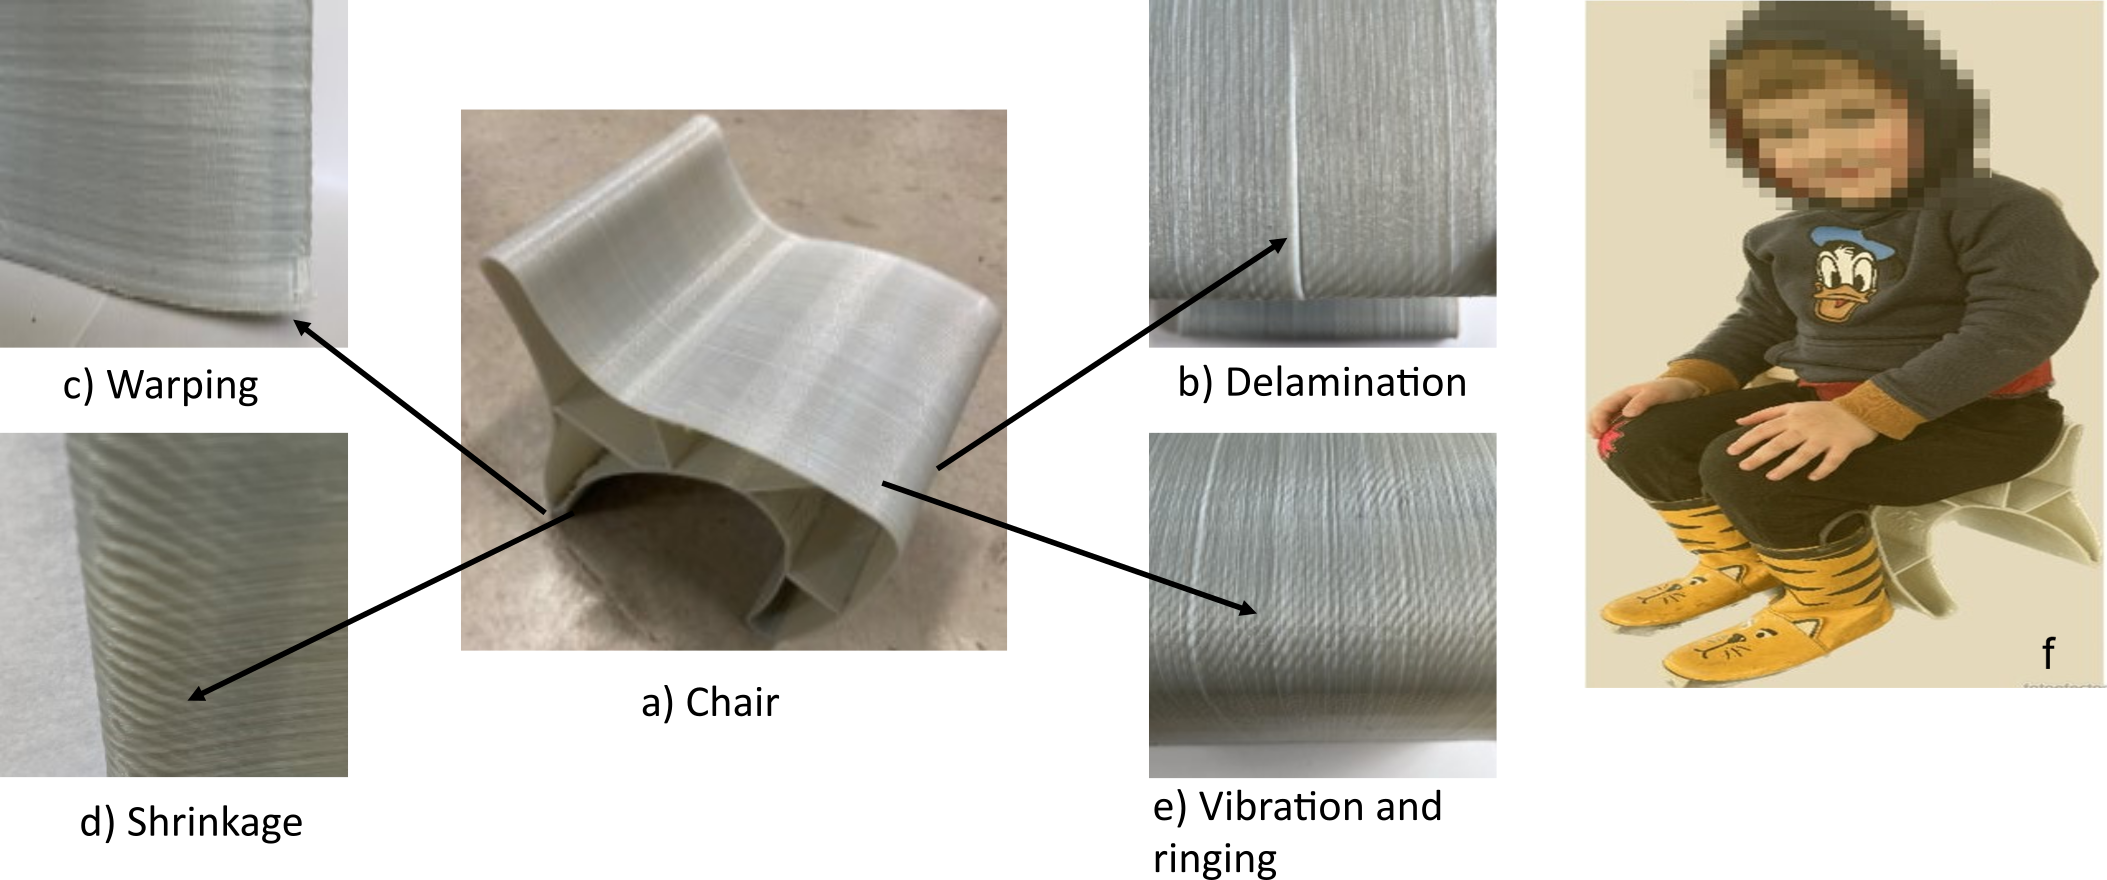
\includegraphics{figures/Figure6.png}

}

\caption{\label{fig-child}Finished children chair and printing issues}

\end{figure}

\hypertarget{cost-and-environmental-impact}{%
\subsubsection{Cost and environmental
impact}\label{cost-and-environmental-impact}}

The printing time took 10 h and the printed object has a mass of 840 g.
Due to the found optimized speed being low, the printing rate ( grams
per hour) is low considering the machine that pellet printers have a
typical throughput of 220 g to 9 kg per hour. The printing time could be
improved by upgrading the extruder motor to a more powerful one.
Besides, the energy required for 10 hr of 3-D printing was found to be 6
kW-hr resulting in a production cost of \textasciitilde1.2 € in function
of the electricity cost in France, without considering the material cost
as bottles were obtained from post-consumers waste. When labor costs are
not included the price was significative reduced (\textasciitilde88\%)
compared with those low cost found in the market.

The economics of fabricating the case study product remained competitive
even if recycled plastic pellets or shreds are used, which can be found
on the market from 1-10 €/kg. However, labor, maintenance and machine
devaluation were not considered in the final price and are needed in
future work for a complete economic evaluation.

Regarding the environmental impact, although this study does not
evaluate the entire life cycle of the printed object, various scientific
studies have already shown feasibility of distributed recycling
(\protect\hyperlink{ref-kerdlap2022}{Kerdlap et al., 2022};
\protect\hyperlink{ref-santander2020}{Santander et al., 2020}), the
comparation between conventional and distributed manufacturing in terms
of energy consumption and emissions
(\protect\hyperlink{ref-Kreiger2013}{Kreiger and Pearce, 2013}),
environmental performance of AM
(\protect\hyperlink{ref-colorado2020a}{Colorado et al., 2020};
\protect\hyperlink{ref-garcia2018}{Garcia et al., 2018}) and the
appearance of DRAM as a source of raw material for diverse 3-D printers
coming from post-consumer plastic waste in the form of either filament
(\protect\hyperlink{ref-hart2018}{Hart et al., 2018};
\protect\hyperlink{ref-mikula2021}{Mikula et al., 2021};
\protect\hyperlink{ref-mohammed2017a}{Mohammed et al., 2017b};
\protect\hyperlink{ref-pakkanen2017}{Pakkanen et al., 2017b}) or
granules (\protect\hyperlink{ref-alexandre2020}{Alexandre et al.,
2020}).

Additionally, Caceres-Mendoza et al.
(\protect\hyperlink{ref-caceres-mendoza2023}{2023}) has developed a
complete life of cycle assessment of a DRAM system based on the
production of PLA filament comparing virgin and recycled materials.
Their environmental results showed a reduction of the impacts of
production (climate change, fossil depletion, water depletion and
potential eutrophication) of \textasciitilde97\% compared to virgin
filament. These results, however, are dependent on the energy supply and
can vary depending on location.

\hypertarget{conclusion-and-future-work}{%
\section{Conclusion and future work}\label{conclusion-and-future-work}}

This study analyzed the feasibility of using mixed post-consumer waste
as feedstock material for direct 3-D printing without compatibilization.
The results showed the potential of mixing solid waste plastics
(PET/HDPE) for its use as feedstock material by printing a water bottle
with two incompatible polymers from the cap and body of the bottle.
Additionally, the results showed that a large-scale FGF 3-D printer was
capable of producing a cost-effective functional object from these mixed
waste PET/HDPE plastics. Further research is needed in the analysis of
mechanical properties of the material as well as the possibilities of
using compatibilizers capable of enhancing the interphase tension
between plastics and lower their crystallinity, which might help improve
performance and enhance material and 3-D printed part properties. These
factors increase in importance as the scale of the 3-D printed part
increases. The improvement of the material science of the approach can
also offer an opportunity to improve the quality of the printing
printing time, lowering the energy consumption of the machine and thus
improving the economic viability of DRAM with mixed plastic waste.

In addition, future work could assess the different types of
combinations or blends between commodity plastics using or not
compatibilizer towards its printability, bringing out the possibility of
selection/sorting process elimination. In the same way, the development
of a methodology that allows the reproducibility of the process even in
areas with limited infrastructure opens up the potential of plastic
revalorization using DRAM.

\hypertarget{declaration-of-competing}{%
\section*{Declaration of competing}\label{declaration-of-competing}}
\addcontentsline{toc}{section}{Declaration of competing}

The authors declare that they have no known competing financial interest
or personal relationships that could have appeared to influence the work
reported in this paper.

\hypertarget{acknowledgements}{%
\section*{Acknowledgements}\label{acknowledgements}}
\addcontentsline{toc}{section}{Acknowledgements}

This project has received funding from the European Union's Horizon 2020
research and innovation program under the grant agreement No 869952. The
authors thank the LUE program for the financing of the thesis, the
Lorraine Fab Living lab platform and the Thompson endowment.

\newpage

\hypertarget{references}{%
\section*{References}\label{references}}
\addcontentsline{toc}{section}{References}

\setstretch{1.1}

\hypertarget{refs}{}
\begin{CSLReferences}{1}{0}
\leavevmode\vadjust pre{\hypertarget{ref-alexandre2020}{}}%
Alexandre, A., Cruz Sanchez, F.A., Boudaoud, H., Camargo, M., Pearce,
J.M., 2020. Mechanical {Properties} of {Direct Waste Printing} of
{Polylactic Acid} with {Universal Pellets Extruder}: {Comparison} to
{Fused Filament Fabrication} on {Open-Source Desktop Three-Dimensional
Printers}. 3D Printing and Additive Manufacturing 7, 237--247.
\url{https://doi.org/10.1089/3dp.2019.0195}

\leavevmode\vadjust pre{\hypertarget{ref-anderson2017}{}}%
Anderson, I., 2017. Mechanical {Properties} of {Specimens 3D Printed}
with {Virgin} and {Recycled Polylactic Acid}. 3D Printing and Additive
Manufacturing 4, 110--115. \url{https://doi.org/10.1089/3dp.2016.0054}

\leavevmode\vadjust pre{\hypertarget{ref-asadi-eydivand2016}{}}%
Asadi-Eydivand, M., Solati-Hashjin, M., Fathi, A., Padashi, M., Abu
Osman, N.A., 2016. Optimal design of a {3D-printed} scaffold using
intelligent evolutionary algorithms. Applied Soft Computing 39, 36--47.
\url{https://doi.org/10.1016/j.asoc.2015.11.011}

\leavevmode\vadjust pre{\hypertarget{ref-attaran2020}{}}%
Attaran, M., 2020. {3D Printing Role} in {Filling} the {Critical Gap} in
the {Medical Supply Chain} during {COVID-19 Pandemic}. American Journal
of Industrial and Business Management 10, 988--1001.
\url{https://doi.org/10.4236/ajibm.2020.105066}

\leavevmode\vadjust pre{\hypertarget{ref-baechler2013}{}}%
Baechler, C., DeVuono, M., Pearce, J.M., 2013. Distributed recycling of
waste polymer into {RepRap} feedstock. Rapid Prototyping Journal 19,
118--125. \url{https://doi.org/10.1108/13552541311302978}

\leavevmode\vadjust pre{\hypertarget{ref-bowyer2014}{}}%
Bowyer, A., 2014. {3D Printing} and {Humanity}'s {First Imperfect
Replicator}. 3D Printing and Additive Manufacturing 1, 4--5.
\url{https://doi.org/10.1089/3dp.2013.0003}

\leavevmode\vadjust pre{\hypertarget{ref-bustosseibert2022}{}}%
Bustos Seibert, M., Mazzei Capote, G.A., Gruber, M., Volk, W., Osswald,
T.A., 2022. Manufacturing of a {PET Filament} from {Recycled Material}
for {Material Extrusion} ({MEX}). Recycling 7, 69.
\url{https://doi.org/10.3390/recycling7050069}

\leavevmode\vadjust pre{\hypertarget{ref-byard2019}{}}%
Byard, D.J., Woern, A.L., Oakley, R.B., Fiedler, M.J., Snabes, S.L.,
Pearce, J.M., 2019. Green fab lab applications of large-area waste
polymer-based additive manufacturing. Additive Manufacturing 27,
515--525. \url{https://doi.org/10.1016/j.addma.2019.03.006}

\leavevmode\vadjust pre{\hypertarget{ref-caceres-mendoza2023}{}}%
Caceres-Mendoza, C., Santander-Tapia, P., Cruz Sanchez, F.A., Troussier,
N., Camargo, M., Boudaoud, H., 2023. Life cycle assessment of filament
production in distributed plastic recycling via additive manufacturing.
Cleaner Waste Systems 5, 100100.
\url{https://doi.org/10.1016/j.clwas.2023.100100}

\leavevmode\vadjust pre{\hypertarget{ref-carrete2021}{}}%
Carrete, I.A., Quiñonez, P.A., Bermudez, D., Roberson, D.A., 2021.
Incorporating {Textile-Derived Cellulose Fibers} for the {Strengthening}
of {Recycled Polyethylene Terephthalate} for {3D Printing Feedstock
Materials}. Journal of polymers and the environment.

\leavevmode\vadjust pre{\hypertarget{ref-chen2015}{}}%
Chen, R.S., Ab Ghani, M.H., Salleh, M.N., Ahmad, S., Tarawneh, M.A.,
2015. Mechanical, water absorption, and morphology of recycled polymer
blend rice husk flour biocomposites. Journal of Applied Polymer Science
132. \url{https://doi.org/10.1002/app.41494}

\leavevmode\vadjust pre{\hypertarget{ref-chong2017}{}}%
Chong, S., Pan, G.-T., Khalid, M., Yang, T.C.-K., Hung, S.-T., Huang,
C.-M., 2017. Physical {Characterization} and {Pre-assessment} of
{Recycled High-Density Polyethylene} as {3D Printing Material}. Journal
of Polymers and the Environment 25, 136--145.
\url{https://doi.org/10.1007/s10924-016-0793-4}

\leavevmode\vadjust pre{\hypertarget{ref-choong2020}{}}%
Choong, Y.Y.C., Tan, H.W., Patel, D.C., Choong, W.T.N., Chen, C.-H.,
Low, H.Y., Tan, M.J., Patel, C.D., Chua, C.K., 2020. The global rise of
3D printing during the {COVID}-19 pandemic. Nat Rev Mater 5, 637--639.
\url{https://doi.org/10.1038/s41578-020-00234-3}

\leavevmode\vadjust pre{\hypertarget{ref-chu2022}{}}%
Chu, J.S., Koay, S.C., Chan, M.Y., Choo, H.L., Ong, T.K., 2022. Recycled
plastic filament made from post-consumer expanded polystyrene and
polypropylene for fused filamant fabrication. Polymer Engineering \&
Science 62, 3786--3795. \url{https://doi.org/10.1002/pen.26144}

\leavevmode\vadjust pre{\hypertarget{ref-cleeman2022}{}}%
Cleeman, J., Bogut, A., Mangrolia, B., Ripberger, A., Kate, K., Zou, Q.,
Malhotra, R., 2022. Scalable, {Flexible} and {Resilient Parallelization}
of {Fused Filament Fabrication}:{Breaking Endemic Tradeoffs} in
{Material Extrusion Additive Manufacturing}. Additive Manufacturing
102926. \url{https://doi.org/10.1016/J.ADDMA.2022.102926}

\leavevmode\vadjust pre{\hypertarget{ref-colorado2020a}{}}%
Colorado, H.A., Velásquez, E.I.G., Monteiro, S.N., 2020. Sustainability
of additive manufacturing: The circular economy of materials and
environmental perspectives. Journal of Materials Research and Technology
9, 8221--8234. \url{https://doi.org/10.1016/j.jmrt.2020.04.062}

\leavevmode\vadjust pre{\hypertarget{ref-corsini2022}{}}%
Corsini, L., Aranda-Jan, C.B., Moultrie, J., 2022. The impact of {3D}
printing on the humanitarian supply chain.
\url{https://doi.org/10.17863/CAM.51226}

\leavevmode\vadjust pre{\hypertarget{ref-cruzsanchez2020}{}}%
Cruz Sanchez, F.A., Boudaoud, H., Camargo, M., Pearce, J.M., 2020.
Plastic recycling in additive manufacturing: {A} systematic literature
review and opportunities for the circular economy. Journal of Cleaner
Production 264, 121602.
\url{https://doi.org/10.1016/j.jclepro.2020.121602}

\leavevmode\vadjust pre{\hypertarget{ref-cruzsanchez2017}{}}%
Cruz Sanchez, F.A., Boudaoud, H., Hoppe, S., Camargo, M., 2017. Polymer
recycling in an open-source additive manufacturing context: {Mechanical}
issues. Additive Manufacturing 17, 87--105.
\url{https://doi.org/10.1016/j.addma.2017.05.013}

\leavevmode\vadjust pre{\hypertarget{ref-dai1997}{}}%
Dai, C.-A., Jandt, K.D., Iyengar, D.R., Slack, N.L., Dai, K.H.,
Davidson, W.B., Kramer, E.J., Hui, C.-Y., 1997. Strengthening {Polymer
Interfaces} with {Triblock Copolymers}. Macromolecules 30, 549--560.
\url{https://doi.org/10.1021/ma960396s}

\leavevmode\vadjust pre{\hypertarget{ref-dertinger2020}{}}%
Dertinger, S.C., Gallup, N., Tanikella, N.G., Grasso, M., Vahid, S.,
Foot, P.J.S., Pearce, J.M., 2020. Technical pathways for distributed
recycling of polymer composites for distributed manufacturing:
{Windshield} wiper blades. Resources, Conservation and Recycling 157,
104810. \url{https://doi.org/10.1016/j.resconrec.2020.104810}

\leavevmode\vadjust pre{\hypertarget{ref-Despeisse2016}{}}%
Despeisse, M., Baumers, M., Brown, P., Charnley, F., Ford, S.J.,
Garmulewicz, A., Knowles, S., Minshall, T.H.W., Mortara, L.,
Reed-Tsochas, F.P., Rowley, J., 2017. Unlocking value for a circular
economy through {3D} printing: {A} research agenda. Technological
Forecasting and Social Change 115, 75--84.
\url{https://doi.org/10.1016/j.techfore.2016.09.021}

\leavevmode\vadjust pre{\hypertarget{ref-evode2021}{}}%
Evode, N., Qamar, S.A., Bilal, M., Barceló, D., Iqbal, H.M.N., 2021.
Plastic waste and its management strategies for environmental
sustainability. Case Studies in Chemical and Environmental Engineering
4, 100142. \url{https://doi.org/10.1016/j.cscee.2021.100142}

\leavevmode\vadjust pre{\hypertarget{ref-fontana2022}{}}%
Fontana, L., Giubilini, A., Arrigo, R., Malucelli, G., Minetola, P.,
2022. Characterization of {3D Printed Polylactic Acid} by {Fused
Granular Fabrication} through {Printing Accuracy}, {Porosity}, {Thermal}
and {Mechanical Analyses}. Polymers 14, 3530.
\url{https://doi.org/10.3390/polym14173530}

\leavevmode\vadjust pre{\hypertarget{ref-Ford2016}{}}%
Ford, S., Despeisse, M., 2016. Additive manufacturing and
sustainability: An exploratory study of the advantages and challenges.
Journal of Cleaner Production 137, 1573--1587.
\url{https://doi.org/10.1016/j.jclepro.2016.04.150}

\leavevmode\vadjust pre{\hypertarget{ref-gaikwad2018}{}}%
Gaikwad, V., Ghose, A., Cholake, S., Rawal, A., Iwato, M., Sahajwalla,
V., 2018. Transformation of {E-Waste Plastics} into {Sustainable
Filaments} for {3D Printing}. ACS Sustainable Chemistry \& Engineering
6, 14432--14440. \url{https://doi.org/10.1021/acssuschemeng.8b03105}

\leavevmode\vadjust pre{\hypertarget{ref-gallup2018}{}}%
Gallup, N., Bow, J.K., Pearce, J.M., 2018. Economic {Potential} for
{Distributed Manufacturing} of {Adaptive Aids} for {Arthritis Patients}
in the {U}.{S}. Geriatrics 3, 89.
\url{https://doi.org/10.3390/geriatrics3040089}

\leavevmode\vadjust pre{\hypertarget{ref-gao2021}{}}%
Gao, X., Qi, S., Kuang, X., Su, Y., Li, J., Wang, D., 2021. Fused
filament fabrication of polymer materials: {A} review of interlayer
bond. Additive Manufacturing 37, 101658.
\url{https://doi.org/10.1016/j.addma.2020.101658}

\leavevmode\vadjust pre{\hypertarget{ref-garcia2018}{}}%
Garcia, F.L., Moris, V.A. da S., Nunes, A.O., Silva, D.A.L., 2018.
Environmental performance of additive manufacturing process
\textendash{} an overview. Rapid Prototyping Journal 24, 1166--1177.
\url{https://doi.org/10.1108/RPJ-05-2017-0108}

\leavevmode\vadjust pre{\hypertarget{ref-geyer2020}{}}%
Geyer, R., 2020. Chapter 2 - {Production}, use, and fate of synthetic
polymers, in: Letcher, T.M. (Ed.), Plastic {Waste} and {Recycling}.
{Academic Press}, pp. 13--32.
\url{https://doi.org/10.1016/B978-0-12-817880-5.00002-5}

\leavevmode\vadjust pre{\hypertarget{ref-Geyer2017}{}}%
Geyer, R., Jambeck, J.R., Law, K.L., 2017. Production, use, and fate of
all plastics ever made. Science Advances 3, e1700782.
\url{https://doi.org/10.1126/sciadv.1700782}

\leavevmode\vadjust pre{\hypertarget{ref-grassi2019}{}}%
Grassi, G., Spagnolo, S.L., Paoletti, I., 2019. Fabrication and
durability testing of a {3D} printed façade for desert climates.
Additive Manufacturing 28, 439.

\leavevmode\vadjust pre{\hypertarget{ref-gwamuri2016}{}}%
Gwamuri, J., Franco, D., Khan, K.Y., Gauchia, L., Pearce, J.M., 2016.
High-{Efficiency Solar-Powered} 3-{D Printers} for {Sustainable
Development}. Machines 4, 3.
\url{https://doi.org/10.3390/machines4010003}

\leavevmode\vadjust pre{\hypertarget{ref-hart2018}{}}%
Hart, K.R., Frketic, J.B., Brown, J.R., 2018. Recycling
meal-ready-to-eat ({MRE}) pouches into polymer filament for material
extrusion additive manufacturing. Additive Manufacturing 21, 536--543.
\url{https://doi.org/10.1016/j.addma.2018.04.011}

\leavevmode\vadjust pre{\hypertarget{ref-imagej2023}{}}%
ImageJ, 2023. Image processing and analysis in java {[}WWW Document{]}.
URL \url{https://imagej.nih.gov/ij/download.html} (accessed 6.13.2023).

\leavevmode\vadjust pre{\hypertarget{ref-inoya2012}{}}%
Inoya, H., Wei Leong, Y., Klinklai, W., Thumsorn, S., Makata, Y.,
Hamada, H., 2012. Compatibilization of recycled poly (ethylene
terephthalate) and polypropylene blends: Effect of polypropylene
molecular weight on homogeneity and compatibility. Journal of applied
polymer science 124, 3947--3955.

\leavevmode\vadjust pre{\hypertarget{ref-jaisinghsheoran2020}{}}%
Jaisingh Sheoran, A., Kumar, H., 2020. Fused {Deposition} modeling
process parameters optimization and effect on mechanical properties and
part quality: {Review} and reflection on present research. Materials
Today: Proceedings, International {Conference} on {Mechanical} and
{Energy Technologies} 21, 1659--1672.
\url{https://doi.org/10.1016/j.matpr.2019.11.296}

\leavevmode\vadjust pre{\hypertarget{ref-jonathanguidigo12017}{}}%
Jonathan GUIDIGO1, Stéphane MOLINA2, Edmond C. ADJOVI3, André MERLIN 4,
DONNOT André5, Merlin SIMO TAGNE6, 2017. Polyethylene {Low} and {High
Density-Polyethylene Terephthalate} and {Polypropylene Blend} as
{Matrices} for {Wood Flour}, in: International {Journal} of {Science}
and {Research} ({IJSR}). pp. 1069--1074.
\url{https://doi.org/10.21275/ART20164296}

\leavevmode\vadjust pre{\hypertarget{ref-jones2011}{}}%
Jones, R., Haufe, P., Sells, E., Iravani, P., Olliver, V., Palmer, C.,
Bowyer, A., 2011. {RepRap} \textendash{} the replicating rapid
prototyper. Robotica 29, 177--191.
\url{https://doi.org/10.1017/S026357471000069X}

\leavevmode\vadjust pre{\hypertarget{ref-kerdlap2022}{}}%
Kerdlap, P., Purnama, A.R., Low, J.S.C., Tan, D.Z.L., Barlow, C.Y.,
Ramakrishna, S., 2022. Comparing the environmental performance of
distributed versus centralized plastic recycling systems: {Applying}
hybrid simulation modeling to life cycle assessment. Journal of
Industrial Ecology 26, 252--271.
\url{https://doi.org/10.1111/jiec.13151}

\leavevmode\vadjust pre{\hypertarget{ref-king2014}{}}%
King, D., Babasola, A., Rozario, J., Pearce, J., 2014. Mobile
{Open-Source Solar-Powered} 3-{D Printers} for {Distributed
Manufacturing} in {Off-Grid Communities}. Challenges in Sustainability
2. \url{https://doi.org/10.12924/cis2014.02010018}

\leavevmode\vadjust pre{\hypertarget{ref-ko2019}{}}%
Ko, Y.S., Herrmann, D., Tolar, O., Elspass, W.J., Brändli, C., 2019.
Improving the filament weld-strength of fused filament fabrication
products through improved interdiffusion. Additive Manufacturing 29,
100815. \url{https://doi.org/10.1016/j.addma.2019.100815}

\leavevmode\vadjust pre{\hypertarget{ref-kramer1994}{}}%
Kramer, E.J., Norton, L.J., Dai, C.-A., Sha, Y., Hui, C.-Y., 1994.
Strengthening polymer interfaces. Faraday Discussions 98, 31--46.
\url{https://doi.org/10.1039/FD9949800031}

\leavevmode\vadjust pre{\hypertarget{ref-kratofil2006}{}}%
Kratofil, L., Hrnjak-Murgić, Z., Jelencć, J., Andricć, B., Kovacć, T.,
Merzel, V., 2006. Study of the compatibilizer effect on blends prepared
from waste poly (ethylene-terephthalate) and high density polyethylene.
International Polymer Processing 21, 328--335.

\leavevmode\vadjust pre{\hypertarget{ref-kreiger2014}{}}%
Kreiger, M.A., Mulder, M.L., Glover, A.G., Pearce, J.M., 2014. Life
cycle analysis of distributed recycling of post-consumer high density
polyethylene for 3-{D} printing filament. Journal of Cleaner Production
70, 90--96. \url{https://doi.org/10.1016/j.jclepro.2014.02.009}

\leavevmode\vadjust pre{\hypertarget{ref-Kreiger2013}{}}%
Kreiger, M., Pearce, J.M., 2013. Environmental {Impacts} of {Distributed
Manufacturing} from 3-{D Printing} of {Polymer Components} and
{Products}. MRS Proceedings 1492, 85--90.
\url{https://doi.org/10.1557/opl.2013.319}

\leavevmode\vadjust pre{\hypertarget{ref-Langer2020}{}}%
Langer, E., Bortel, K., Waskiewicz, S., Lenartowicz-Klik, M., 2020.
Methods of {PET Recycling}, Plasticizers Derived from Post-Consumer PET.
\url{https://doi.org/10.1016/b978-0-323-46200-6.00005-2}

\leavevmode\vadjust pre{\hypertarget{ref-lei2009}{}}%
Lei, Y., Wu, Q., Zhang, Q., 2009. Morphology and properties of
microfibrillar composites based on recycled poly (ethylene
terephthalate) and high density polyethylene. Composites Part A: Applied
Science and Manufacturing 40, 904--912.
\url{https://doi.org/10.1016/j.compositesa.2009.04.017}

\leavevmode\vadjust pre{\hypertarget{ref-lipsky2019}{}}%
Lipsky, S., Przyjemski, A., Velasquez, M., Gershenson, J., 2019. {3D
Printing} for {Humanitarian Relief}: {The Printer Problem}, in: 2019
{IEEE Global Humanitarian Technology Conference} ({GHTC}). pp. 1--7.
\url{https://doi.org/10.1109/GHTC46095.2019.9033053}

\leavevmode\vadjust pre{\hypertarget{ref-little2020}{}}%
Little, H.A., Tanikella, N.G., J. Reich, M., Fiedler, M.J., Snabes,
S.L., Pearce, J.M., 2020. Towards {Distributed Recycling} with {Additive
Manufacturing} of {PET Flake Feedstocks}. Materials 13, 4273.
\url{https://doi.org/10.3390/ma13194273}

\leavevmode\vadjust pre{\hypertarget{ref-loschke2019}{}}%
Löschke, S.K., Mai, J., Proust, G., Brambilla, A., 2019. Microtimber:
{The Development} of a {3D Printed Composite Panel Made} from {Waste
Wood} and {Recycled Plastics}. Digital Wood Design 24, 827--848.
\url{https://doi.org/10.1007/978-3-030-03676-8_33}

\leavevmode\vadjust pre{\hypertarget{ref-macarthur2017}{}}%
MacArthur, E., 2017. Beyond plastic waste. Science 358, 843--843.
\url{https://doi.org/10.1126/science.aao6749}

\leavevmode\vadjust pre{\hypertarget{ref-mikula2021}{}}%
Mikula, K., Skrzypczak, D., Izydorczyk, G., Warchoł, J., Moustakas, K.,
Chojnacka, K., Witek-Krowiak, A., 2021. {3D} printing filament as a
second life of waste plastics\textemdash a review. Environmental Science
and Pollution Research 28, 12321--12333.
\url{https://doi.org/10.1007/s11356-020-10657-8}

\leavevmode\vadjust pre{\hypertarget{ref-mohammed2017}{}}%
Mohammed, M.I., Das, A., Gomez-Kervin, E., Wilson, D., Gibson, I.,
2017a. {EcoPrinting}: {Investigating} the {Use} of 100\% {Recycled
Acrylonitrile Butadiene Styrene} ({ABS}) for {Additive Manufacturing}.
{University of Texas at Austin}.

\leavevmode\vadjust pre{\hypertarget{ref-mohammed2017a}{}}%
Mohammed, M.I., Mohan, M., Das, A., Johnson, M.D., Badwal, P.S., McLean,
D., Gibson, I., 2017b. A low carbon footprint approach to the
reconstitution of plastics into {3D-printer} filament for enhanced waste
reduction. KnE Engineering 234--241.
\url{https://doi.org/10.18502/keg.v2i2.621}

\leavevmode\vadjust pre{\hypertarget{ref-Mohammed2018}{}}%
Mohammed, M.I., Wilson, D., Gomez-Kervin, E., Rosson, L., Long, J.,
2018. {EcoPrinting}: {Investigation} of {Solar Powered Plastic
Recycling} and {Additive Manufacturing} for {Enhanced Waste Management}
and {Sustainable Manufacturing}, in: 2018 {IEEE Conference} on
{Technologies} for {Sustainability} ({SusTech}). {IEEE}, pp. 1--6.
\url{https://doi.org/10.1109/SusTech.2018.8671370}

\leavevmode\vadjust pre{\hypertarget{ref-nofar2019}{}}%
Nofar, M., Oğuz, H., 2019. Development of {PBT}/{Recycled-PET Blends}
and the {Influence} of {Using Chain Extender}. Journal of Polymers and
the Environment 27, 1404--1417.
\url{https://doi.org/10.1007/s10924-019-01435-w}

\leavevmode\vadjust pre{\hypertarget{ref-novak2020}{}}%
Novak, J.I., Loy, J., 2020. A critical review of initial {3D} printed
products responding to {COVID-19} health and supply chain challenges.
Emerald Open Research 2, 24.
\url{https://doi.org/10.35241/emeraldopenres.13697.1}

\leavevmode\vadjust pre{\hypertarget{ref-oberloier2022}{}}%
Oberloier, S., Whisman, N.G., Pearce, J.M., 2022a. Finding {Ideal
Parameters} for {Recycled Material Fused Particle Fabrication-Based 3D
Printing Using} an {Open Source Software Implementation} of {Particle
Swarm Optimization}. 3D Printing and Additive Manufacturing.
\url{https://doi.org/10.1089/3dp.2022.0012}

\leavevmode\vadjust pre{\hypertarget{ref-oberloier2022a}{}}%
Oberloier, S., Whisman, N.G., Pearce, J.M., 2022b. Finding {Ideal
Parameters} for {Recycled Material Fused Particle Fabrication-Based 3D
Printing Using} an {Open Source Software Implementation} of {Particle
Swarm Optimization}. 3D Printing and Additive Manufacturing.
\url{https://doi.org/10.1089/3dp.2022.0012}

\leavevmode\vadjust pre{\hypertarget{ref-Pakkanen2017}{}}%
Pakkanen, J., Manfredi, D., Minetola, P., Iuliano, L., 2017a. About the
{Use} of {Recycled} or {Biodegradable Filaments} for {Sustainability} of
{3D Printing}, in: Campana, G., Howlett, R.J., Setchi, R., Cimatti, B.
(Eds.),. {Springer International Publishing}, {Cham}, pp. 776--785.
\url{https://doi.org/10.1007/978-3-319-57078-5_73}

\leavevmode\vadjust pre{\hypertarget{ref-pakkanen2017}{}}%
Pakkanen, J., Manfredi, D., Minetola, P., Iuliano, L., 2017b. About the
{Use} of {Recycled} or {Biodegradable Filaments} for {Sustainability} of
{3D Printing}, in: Campana, G., Howlett, R.J., Setchi, R., Cimatti, B.
(Eds.), Sustainable {Design} and {Manufacturing} 2017, Smart
{Innovation}, {Systems} and {Technologies}. {Springer International
Publishing}, {Cham}, pp. 776--785.
\url{https://doi.org/10.1007/978-3-319-57078-5_73}

\leavevmode\vadjust pre{\hypertarget{ref-pan2020}{}}%
Pan, Y., Wu, G., Ma, H., Zhou, S., Zhang, H., 2020. Improved
compatibility of PET/HDPE blend by using GMA grafted thermoplastic
elastomer. Polymer-Plastics Technology and Materials 59, 1887--1898.

\leavevmode\vadjust pre{\hypertarget{ref-pearce2022}{}}%
Pearce, J., Qian, J.-Y., 2022. Economic {Impact} of {DIY Home
Manufacturing} of {Consumer Products} with {Low-cost 3D Printing} from
{Free} and {Open Source Designs}. European Journal of Social Impact and
Circular Economy 3, 1--24. \url{https://doi.org/10.13135/2704-9906/6508}

\leavevmode\vadjust pre{\hypertarget{ref-Petersen2017}{}}%
Petersen, E., Kidd, R., Pearce, J., 2017. Impact of {DIY Home
Manufacturing} with {3D Printing} on the {Toy} and {Game Market}.
Technologies 5, 45. \url{https://doi.org/10.3390/technologies5030045}

\leavevmode\vadjust pre{\hypertarget{ref-petsiuk2022}{}}%
Petsiuk, A., Lavu, B., Dick, R., Pearce, J.M., 2022. Waste {Plastic
Direct Extrusion Hangprinter}. Inventions 7, 70.
\url{https://doi.org/10.3390/inventions7030070}

\leavevmode\vadjust pre{\hypertarget{ref-pringle2018}{}}%
Pringle, A.M., Rudnicki, M., Pearce, J.M., 2018. Wood {Furniture
Waste}\textendash{{Based Recycled}} 3-{D Printing Filament}. Forest
Products Journal 68, 86--95.
\url{https://doi.org/10.13073/FPJ-D-17-00042}

\leavevmode\vadjust pre{\hypertarget{ref-raju2019}{}}%
Raju, M., Gupta, M.K., Bhanot, N., Sharma, V.S., 2019. A hybrid
{PSO}\textendash{{BFO}} evolutionary algorithm for optimization of fused
deposition modelling process parameters. Journal of Intelligent
Manufacturing 30, 2743--2758.
\url{https://doi.org/10.1007/s10845-018-1420-0}

\leavevmode\vadjust pre{\hypertarget{ref-rattan2023}{}}%
Rattan, R.S., Nauta, N., Romani, A., Pearce, J.M., 2023. Hangprinter for
large scale additive manufacturing using fused particle fabrication with
recycled plastic and continuous feeding. HardwareX 13, e00401.
\url{https://doi.org/10.1016/j.ohx.2023.e00401}

\leavevmode\vadjust pre{\hypertarget{ref-reich2019b}{}}%
Reich, M.J., Woern, A.L., Tanikella, N.G., Pearce, J.M., 2019.
Mechanical {Properties} and {Applications} of {Recycled Polycarbonate
Particle Material Extrusion-Based Additive Manufacturing}. Materials 12,
1642. \url{https://doi.org/10.3390/ma12101642}

\leavevmode\vadjust pre{\hypertarget{ref-rett2021}{}}%
Rett, J.P., Traore, Y.L., Ho, E.A., 2021. Sustainable {Materials} for
{Fused Deposition Modeling 3D Printing Applications}. Advanced
Engineering Materials 23, 2001472.
\url{https://doi.org/10.1002/adem.202001472}

\leavevmode\vadjust pre{\hypertarget{ref-romani2021}{}}%
Romani, A., Rognoli, V., Levi, M., 2021. Design, {Materials}, and
{Extrusion-Based Additive Manufacturing} in {Circular Economy Contexts}:
{From Waste} to {New Products}. Sustainability 13, 7269.
\url{https://doi.org/10.3390/su13137269}

\leavevmode\vadjust pre{\hypertarget{ref-roschli2019}{}}%
Roschli, A., Gaul, K.T., Boulger, A.M., Post, B.K., Chesser, P.C., Love,
L.J., Blue, F., Borish, M., 2019. Designing for {Big Area Additive
Manufacturing}. Additive Manufacturing 25, 275--285.
\url{https://doi.org/10.1016/j.addma.2018.11.006}

\leavevmode\vadjust pre{\hypertarget{ref-saad2019a}{}}%
Saad, M.S., Nor, A.M., Baharudin, M.E., Zakaria, M.Z., Aiman, A.F.,
2019. Optimization of surface roughness in {FDM 3D} printer using
response surface methodology, particle swarm optimization, and symbiotic
organism search algorithms. The International Journal of Advanced
Manufacturing Technology 105, 5121--5137.
\url{https://doi.org/10.1007/s00170-019-04568-3}

\leavevmode\vadjust pre{\hypertarget{ref-salmi2020}{}}%
Salmi, M., Akmal, J.S., Pei, E., Wolff, J., Jaribion, A., Khajavi, S.H.,
2020. {3D Printing} in {COVID-19}: {Productivity Estimation} of the
{Most Promising Open Source Solutions} in {Emergency Situations}.
Applied Sciences 10, 4004. \url{https://doi.org/10.3390/app10114004}

\leavevmode\vadjust pre{\hypertarget{ref-santander2020}{}}%
Santander, P., Cruz Sanchez, F.A., Boudaoud, H., Camargo, M., 2020.
Closed loop supply chain network for local and distributed plastic
recycling for {3D} printing: A {MILP-based} optimization approach.
Resources, Conservation and Recycling 154, 104531.
\url{https://doi.org/10.1016/j.resconrec.2019.104531}

\leavevmode\vadjust pre{\hypertarget{ref-savonen2018}{}}%
Savonen, B.L., Mahan, T.J., Curtis, M.W., Schreier, J.W., Gershenson,
J.K., Pearce, J.M., 2018. Development of a {Resilient} 3-{D Printer} for
{Humanitarian Crisis Response}. Technologies 6, 30.
\url{https://doi.org/10.3390/technologies6010030}

\leavevmode\vadjust pre{\hypertarget{ref-schirmeister2019}{}}%
Schirmeister, C.G., Hees, T., Licht, E.H., Mülhaupt, R., 2019. {3D}
printing of high density polyethylene by fused filament fabrication.
Additive Manufacturing 28, 152--159.
\url{https://doi.org/10.1016/j.addma.2019.05.003}

\leavevmode\vadjust pre{\hypertarget{ref-sells2009}{}}%
Sells, E., Smith, Z., Bailard, S., Bowyer, A., Olliver, V., 2009.
{RepRap}: {The Replicating Rapid Prototyper} - maximizing
customizability by breeding the means of production, in: Piller, F.T.,
Tseng, M.M. (Eds.), Handbook of {Research} in {Mass Customization} and
{Personalization}. {World Scientific}, pp. 568--580.

\leavevmode\vadjust pre{\hypertarget{ref-selvam2020}{}}%
Selvam, A., Mayilswamy, S., Whenish, R., 2020. Strength {Improvement} of
{Additive Manufacturing Components} by {Reinforcing Carbon Fiber} and by
{Employing Bioinspired Interlock Sutures}. Journal of Vinyl and Additive
Technology 26, 511--523. \url{https://doi.org/10.1002/vnl.21766}

\leavevmode\vadjust pre{\hypertarget{ref-shah2019}{}}%
Shah, J., Snider, B., Clarke, T., Kozutsky, S., Lacki, M., Hosseini, A.,
2019. Large-scale {3D} printers for additive manufacturing: Design
considerations and challenges. The International Journal of Advanced
Manufacturing Technology 104, 3679--3693.
\url{https://doi.org/10.1007/s00170-019-04074-6}

\leavevmode\vadjust pre{\hypertarget{ref-shirmohammadi2021}{}}%
Shirmohammadi, M., Goushchi, S.J., Keshtiban, P.M., 2021. Optimization
of {3D} printing process parameters to minimize surface roughness with
hybrid artificial neural network model and particle swarm algorithm.
Progress in Additive Manufacturing 6, 199--215.
\url{https://doi.org/10.1007/s40964-021-00166-6}

\leavevmode\vadjust pre{\hypertarget{ref-Siltaloppi2021}{}}%
Siltaloppi, J., Jähi, M., 2021. Toward a sustainable plastics value
chain: {Core} conundrums and emerging solution mechanisms for a systemic
transition. Journal of Cleaner Production 315, 128113.
\url{https://doi.org/10.1016/j.jclepro.2021.128113}

\leavevmode\vadjust pre{\hypertarget{ref-soares2021}{}}%
Soares, J., Miguel, I., Venâncio, C., Lopes, I., Oliveira, M., 2021.
Public views on plastic pollution: {Knowledge}, perceived impacts, and
pro-environmental behaviours. Journal of Hazardous Materials 412,
125227. \url{https://doi.org/10.1016/j.jhazmat.2021.125227}

\leavevmode\vadjust pre{\hypertarget{ref-taghavi2018}{}}%
Taghavi, S.K., Shahrajabian, H., Hosseini, H.M., 2018. Detailed
comparison of compatibilizers MAPE and SEBS-g-MA on the
mechanical/thermal properties, and morphology in ternary blend of
recycled PET/HDPE/MAPE and recycled PET/HDPE/SEBS-g-MA. Journal of
Elastomers \& Plastics 50, 13--35.

\leavevmode\vadjust pre{\hypertarget{ref-vandevoorde2022}{}}%
Van de Voorde, B., Katalagarianakis, A., Huysman, S., Toncheva, A.,
Raquez, J.-M., Duretek, I., Holzer, C., Cardon, L., Bernaerts, K., V,
Van Hemelrijck, D., Pyl, L., Van Vlierberghe, S., 2022. Effect of
extrusion and fused filament fabrication processing parameters of
recycled poly(ethylene terephthalate) on the crystallinity and
mechanical properties. Additive Manufacturing 50.
\url{https://doi.org/10.1016/j.addma.2021.102518}

\leavevmode\vadjust pre{\hypertarget{ref-vaucher2022}{}}%
Vaucher, J., Demongeot, A., Michaud, V., Leterrier, Y., 2022. Recycling
of {Bottle Grade PET}: {Influence} of {HDPE Contamination} on the
{Microstructure} and {Mechanical Performance} of {3D Printed Parts}.
Polymers 14, 5507. \url{https://doi.org/10.3390/polym14245507}

\leavevmode\vadjust pre{\hypertarget{ref-verma2023}{}}%
Verma, N., Awasthi, P., Gupta, A., Banerjee, S.S., 2023. Fused
{Deposition Modeling} of {Polyolefins}: {Challenges} and
{Opportunities}. Macromolecular Materials and Engineering 308, 2200421.
\url{https://doi.org/10.1002/mame.202200421}

\leavevmode\vadjust pre{\hypertarget{ref-wijnen2018}{}}%
Wijnen, B., Sanders, P., Pearce, J.M., 2018. Improved model and
experimental validation of deformation in fused filament fabrication of
polylactic acid. Progress in Additive Manufacturing 3, 193--203.
\url{https://doi.org/10.1007/s40964-018-0052-4}

\leavevmode\vadjust pre{\hypertarget{ref-william2021}{}}%
William, L.J.W., Koay, S.C., Chan, M.Y., Pang, M.M., Ong, T.K., Tshai,
K.Y., 2021. Recycling {Polymer Blend} made from {Post-used Styrofoam}
and {Polypropylene} for {Fuse Deposition Modelling}. Journal of Physics:
Conference Series 2120, 012020.
\url{https://doi.org/10.1088/1742-6596/2120/1/012020}

\leavevmode\vadjust pre{\hypertarget{ref-woern2018}{}}%
Woern, A.L., McCaslin, J.R., Pringle, A.M., Pearce, J.M., 2018.
{RepRapable Recyclebot}: {Open} source 3-{D} printable extruder for
converting plastic to 3-{D} printing filament. HardwareX 4, e00026.
\url{https://doi.org/10.1016/j.ohx.2018.e00026}

\leavevmode\vadjust pre{\hypertarget{ref-wong2015}{}}%
Wong, J.Y., 2015. Ultra-{Portable Solar-Powered 3D Printers} for {Onsite
Manufacturing} of {Medical Resources}. Aerospace Medicine and Human
Performance 86, 830--834. \url{https://doi.org/10.3357/AMHP.4308.2015}

\leavevmode\vadjust pre{\hypertarget{ref-Zander2019}{}}%
Zander, N.E., Gillan, M., Burckhard, Z., Gardea, F., 2019. Recycled
polypropylene blends as novel {3D} printing materials. Additive
Manufacturing 25, 122--130.
\url{https://doi.org/10.1016/j.addma.2018.11.009}

\leavevmode\vadjust pre{\hypertarget{ref-zander2018}{}}%
Zander, N.E., Gillan, M., Lambeth, R.H., 2018. Recycled polyethylene
terephthalate as a new {FFF} feedstock material. Additive Manufacturing
21, 174--182. \url{https://doi.org/10.1016/j.addma.2018.03.007}

\leavevmode\vadjust pre{\hypertarget{ref-zhang2015}{}}%
Zhang, Y., Wang, S., Ji, G., 2015. A {Comprehensive Survey} on {Particle
Swarm Optimization Algorithm} and {Its Applications}. Mathematical
Problems in Engineering 2015, e931256.
\url{https://doi.org/10.1155/2015/931256}

\leavevmode\vadjust pre{\hypertarget{ref-zhong2018}{}}%
Zhong, S., Pearce, J.M., 2018. Tightening the loop on the circular
economy: {Coupled} distributed recycling and manufacturing with
recyclebot and {RepRap} 3-{D} printing. Resources, Conservation and
Recycling 128, 48--58.
\url{https://doi.org/10.1016/j.resconrec.2017.09.023}

\end{CSLReferences}



\end{document}
